%!TEX root = ../../thesis.tex

\graphicspath{{Chapters/spider/figures/}}

\chapter{SpiderNet}\label{chapter:spider}
\section{Introduction}\label{sect:spider_intro}
While BonsaiNet reliably produces good models within a given configuration, its search flexibility is implicitly limited by
its configuration, specifically by the need to specify the per-cell node count and depth. While the operations between
these specified nodes can vary, the actual edge structure of any cell is fixed. Therefore, there is a significant
measure of human design and intuition necessary to choose ideal node and depth parameters, or barring that, a lot of
brute force experimentation. This feels rather counterintuitive to the general point of neural architecture search, which
strives to eliminate the need for finicky intuition or hyperparameter grid searches. Arguably, these algorithms
that rely on user configuration of the final structural connectivity are just moving the burden of search one level
higher, replacing architecture search with \textit{architecture-search} search. To this end, what is the point of reporting that
a NAS algorithm can produce an amazing architecture in a few GPU-hours, if it takes a dozen tries to figure
out how to configure said algorithm?

With that question in mind, it is of interest to explore
models that approached the model growth problem from the opposite direction; rather than specify the structure of the initial
supernet and use Bonsai to find some optimal subnet, the goal was to start with some minimum viable model and allow the model
to dynamically expand the search space as it saw fit. By letting the model choose its own overall structure as well
as the specifics of its connectivity, in theory the flexibility and ease-of-applicability of
NAS could be greatly improved.

In this chapter, Section~\ref{sect:spiderbackground} will first cover some necessary background material.
Section~\ref{sect:spiderdesign} will next cover the components and general design of SpiderNet,
an algorithm that meets these specifications. Next, Section~\ref{sect:spider_tf_mutations} will cover the neural network
theory that is used to calculate SpiderNet's operational heuristics. With design and theory covered, the full SpiderNet
algorithm is stated in Section~\ref{sect:spider_alg}. Various experimental designs over this algorithm are described in
Section~\ref{sect:spider_experiments}, the results of which are discussed in Sections~\ref{sect:spider_results} and~\ref{sect:spider_discussion}. Finally,
Section~\ref{sect:spider_futurework} explores some open questions around SpiderNet, before wrapping up in Section~\ref{sect:spider_conclusion}.

\section{Background}\label{sect:spiderbackground}
To understand certain specific components of SpiderNet, two concepts must first be discussed: SHAP and train-free model metrics.

\subsection{SHAP}\label{sect:spiderbackgroundshap}
SHAP or SHapley Additive exPlanations was introduced by~\cite{lundberg2017} as a means of adapting game theory's
Shapley value into an explainable AI context. Shapley values are a measure of an individual's
contribution to a coalition, where a coalition is a group of cooperating members and
the value of a coalition $C$ is defined as some function $F$ with respect to its members. The Shapley value of an individual
is calculated by computing the mean difference in coalition value between
each pair of coalition permutations that differ only by the inclusion of that particular individual:
\begin{align}
    \phi_i = \frac{1}{\text{\# coalition members}} \sum_{\text{all coalitions}\;C\;\text{excluding i}} \frac{F(C\bigcup i) - F(C)}{\text{\# coalitions excluding}\;i\;\text{of size}\;|C|},
\end{align}
where $F(C\bigcup i)$ is the coalition value of the coalition formed by adding member $i$ to coalition $C$, ``all coalitions $C$ excluding i''
refers to every possible permutation of the available coalition members that excludes member $i$, and ``\# coalitions excluding $i$ of size $|C|$''
refers to the total number of coalition permutations that exclude member $i$ but have an equal number of members as $C$.

For example, given some coalition that consists of three members Isabelle, James, and Kate, Isabelle's Shapley value $\phi_{I}$ can be calculated
by first enumerating the following values for each of the four coalitions $C$ that exclude Isabelle:

\begin{center}
\begin{tabular}{c|ccc}
         Coalition $C$  & $F(C\bigcup i)$   &  $F(C)$           & Coalitions excluding $i$ of size $|C|$ \\ \hline
         $(J,K)$          & F(I, J, K)        & F(J, K)           & (J, K) \\
         $(J)$            & F(I, J)           & F(J)              & (J), (K) \\
         $(K)$            & F(I, K)           & F(K)              & (J), (K) \\
         $(\varnothing)$  & F(I)              & $F(\varnothing)$  & $(\varnothing)$ \\
\end{tabular}
\end{center}
\noindent Therefore:
\begin{align*}
    \phi_{\text{Isabelle}} = \frac{1}{4} \left(\frac{F(I, J, K) - F(J, K)}{1} + \frac{F(I, J) - F(J)}{2} + \frac{F(I, K) - F(K)}{2} + \frac{F(I) - F(\varnothing)}{1} \right)
\end{align*}

The Shapley values can then be used to model coalition value additively, such that:
\begin{align}
    F(C) = F(\varnothing) + \sum_{i=1}^N \phi_i x_i
\end{align}
\noindent where $x_i$ is a binary value that indicates the presence or absence of the $ith$ member of the coalition $C$.
Under this formulation, $\phi_i$ gives the exact contribution that member $i$ had on the coalition value $F(C)$.

To adapt this concept from game theory to explainable AI,~\cite{lundberg2017} uses a model's input features
as the coalition and the model's output as a coalition value, and therefore the Shapley value $\phi_i$ would
model how much a feature $i$ affected the model's output value. To avoid needing to sample massive numbers of
coalition pairs when explaining many-feature models,~\citeauthor{lundberg2017} devise a sampling algorithm that uses a weighted linear
regression to recover the Shapley values of features with exponentially fewer samples than raw computation of Shapley
values would require. Additionally, they create a formulation to mathematically approximate the effects of removing input features
without needing to reformulate models that may not allow for variable-length inputs. From this, SHAP can
provide an easily interpretable explanation as to how the inputs $\vec{x}$ to a model $M$ affected $M(\vec{x})$, simply by looking at
$\phi_0, \dots, \phi_n$.


\subsection{Train-Free Metrics}
A train-free metric refers to methods that evaluate a model's quality via sampling methods that involve
no backpropagation or weight sampling, ideally in such a way that the metric correlates strongly with final
model performance. Two model characteristics that train-free metrics commonly seek to quantify are
\textit{trainability} and \textit{expressability}.

Trainability refers to the effectiveness of gradient descent at optimizing
a model. This factor is one of the reasons for performance differences between models of vastly different parameter counts;
for example, VGGNet-E has 144M parameters and scores a 74.5\% top-1 test accuracy on ImageNet, while ResNet-152 has less
than half at 60.1M yet scores a 80.62\%~\citep{simon2014,he2015}. Trainability lets us explain this disparity; the
ResNet is more trainable than the VGGNet, which lets it use its parameters more effectively and efficiently which more
than makes up for its lower parameter count. Expressability, on the other hand, refers to the complexity of function that the model can approximate. Expressability
is the culprit behind the bigger-is-better phenomena seen in ResNets or VGGNets; with more parameters, the bigger models
can approximate more complex functions (and therefore have higher expressability) and thus tend to perform better. Of course,
expressability is more complex than just parameter count, as a model's operations and their interactions are very important to the
nature of the functions the model can represent. These two measures are best used in combination, as the best models
will have both high trainability and expressability; that is, they easily reach their full potential and that full potential is powerful.

One such paper that applies train-free metrics to a NAS context is~\cite{chen2021}, titled
\hyperlink{cite.chen2021}{``Neural Architecture Search on ImageNet in Four GPU Hours: A Theoretically Inspired Perspective''}. This paper explores
the use of two train-free metrics, the neural tangent kernel and linear region count,
as means trainability and expressability respectively. These are then used to differentiate between different models
in a search space to rapidly speed up the search process.


\subsection{Neural Tangent Kernel}\label{sect:ntk_intro}
 To measure trainability, \citeauthor{chen2021} use~\citeauthor{jacot2018}'s
\textit{Neural Tangent Kernel} or NTK, which is used to analytically model the training dynamics of neural networks
through differential equations. The exact derivation of the NTK is complex and not relevant to the discussion here, but
in summary the derivation is based around observing network training dynamics, approximating the network as a linear
function through Taylor expansion and analytically representing the dynamics of that approximation's output as
an ordinary differential equation~\citep{dwaraknath2014}. This differential equation of training dynamics ends up being a function of
the pairwise inner product of the \textit{feature maps} of a model at initialization, where feature map is defined as:
\begin{align}
    \phi = \nabla_\theta f(\mathbf{X}, \theta_0)
\end{align}
\noindent This $\phi$ is a matrix, where $\phi_{i,j}$ is the gradient of the $i$th parameter given the $j$th input datapoint and the
initial state of the model parameters $\theta_0$, thus measuring the direction and magnitude of change of each parameter in the model
given the entirety of the training data $\mathbf{X}$. The pairwise inner product $\phi^T\phi$ represented by $\Phi$ therefore gives the dot product
of the column vectors $\phi_{*,i}$ and $\phi_{*,j}$ for all pairs $i, j$:
\begin{align}
    \Phi_{i,j} &= \phi^T_{i,0}\phi_{0,j} + \phi_{i,1}T\phi_{1,j} + \dots + \phi_{i,p}^T\phi_{p,j} \\
               &= \phi_{0,i}\phi_{0,j}   + \phi_{1,i}\phi_{1,j}   + \dots + \phi_{p,i}\phi_{p,j}
\end{align}
\noindent Therefore, the $i$th element of the diagonal $\Phi_{i,i}$ gives the sum of the squared gradient of each
parameter in the model induced by the $i$th datapoint, which measures the magnitude of the training contribution of that
particular datapoint between initialization and some arbitrary point in the model's future. Specifically, this product is
\begin{align}
    \frac{\partial f(\mathbf{X}, \theta_t)}{\partial t} &= -\Phi (f(\mathbf{X}, \theta_t) - \mathbf{Y})
\end{align}
\noindent where $\theta_t$ are the model parameters at some time $t$, $f(\mathbf{X}, \theta_t)$ is the model
output over the training inputs given the parameter values $\theta_t$,
and $\mathbf{Y}$ are the correct training labels
of the data.
A situation where $f(\mathbf{X}, \theta_t) = \mathbf{Y}$ represents model convergence and perfect train accuracy, which is always the target
of training. By replacing $f(\mathbf{X}, \theta_t) - \mathbf{Y}$ with $u$, the above differential equations can be solved as:
\begin{align}
    u(t) = u(0) e^{-\Phi t}
\end{align}
Since $u(t)=0$ represents convergence and $u(0)$ is the initial state of the model, the fully-trained state of the model
is attained once the initial state $u(0)$ fully decays to 0. The exponential rate of this decay is thus governed
by $\Phi$. By performing a spectral decomposition of $\Phi$, this can be written as:
\begin{align}
    u(t) &= u(0) e^{-t Q\Lambda Q^{-1}} \\
         &= u(0) Q e^{-t \Lambda} Q^{-1}
\end{align}
Since $\Lambda$ is a diagonal matrix of eigenvalues, it is then possible to define $e^{-t \Lambda}=\Lambda'$, where $\Lambda'$ is a diagonal
matrix with $\Lambda'_{i,i}=e^{-t \lambda_i}$. Therefore, the decay of the initial state into the converged
state can be represented as a linear combination of exponential decays along each eigenvector, the rates of which are given by the
corresponding eigenvalues $\lambda$. The thing that makes all of this so useful is that the matrix $\Phi$ is invariant with respect to time (i.e., training steps)
if the actual model is relatively close to its linear Taylor-expanded representation~\citep{dwaraknath2014}.
This means that the relative rate of training convergence can be measured using these eigenvalues, without needing to
perform any training on the model whatsoever. \citeauthor{chen2021} choose to mark the largest eigenvalue as $\lambda_0$
and the smallest as $\lambda_m$, and use these to define $\kappa = \frac{\lambda_0}{\lambda_m}$ as their relative measure of trainability.
Large $\kappa$ values indicate that the model converges much more quickly along certain directions versus others, while a low
$\kappa$ value indicates more uniform convergence along all directions.

In practice, the measurement of NTK is highly expensive: the $\Phi$ matrix needs an equal number of rows as parameters in
the model, which means its construction can be prohibitively large on any meaningfully sized model. To account for this,
\citeauthor{chen2021} use a ``slim'' version of the candidate model as a proxy for the full model's NTK. This slim model
only has a single channel throughout; each convolution operation only has a single kernel and all operations operate
exclusively in monochrome. The idea is that the NTK of this single-sliced model will adequately approximate the NTK
of the full model. However, this is never justified or even mentioned in the original paper,
only from investigating the source code did I uncover this approximation.

Regardless, \citeauthor{chen2021} provide a proof-of-concept of their NTK measurements through analysis of the models within
NAS-Bench-201~\citep{dong2020}, a collection of 15,625 different
neural architectures and their corresponding CIFAR-100 performances. By determining the $\kappa$ value of all 15,625 models
at initialization, they find a strong negative correlation with final test accuracy, with a Kendall-tau correlation
of -0.42. The full results of their study are shown in Figure~\ref{fig:ntk}:

\begin{figure}[ht]
    \centering
	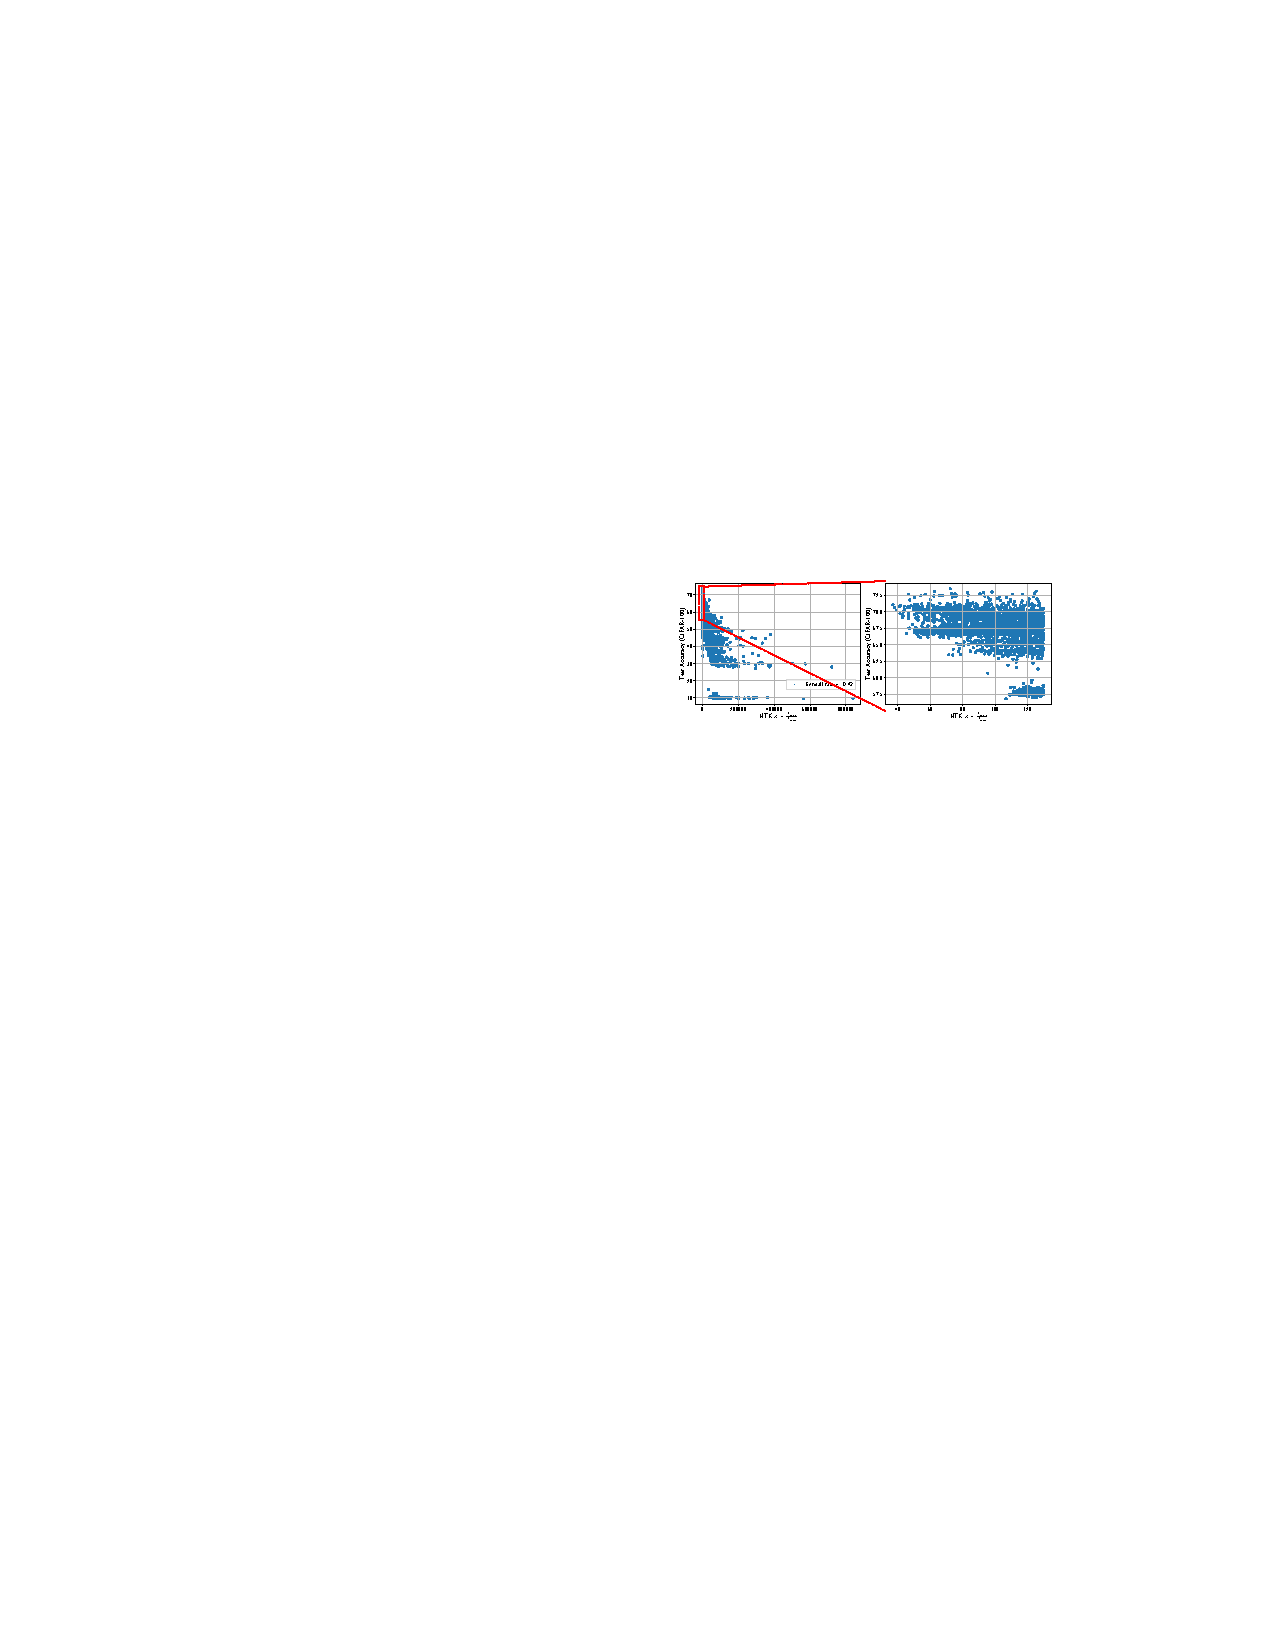
\includegraphics[width=\textwidth]{ntk} \\
	\caption[The correlation between $\kappa$ and CIFAR-100 test accuracy]{The correlation between $\kappa$ and CIFAR-100 test accuracy, as shown in~\cite{chen2021}. The left
    plot shows all 15,625 models, while the right plot zooms in on the narrow rectangular region highlighted in red.
    The two horiztonal dashed lines are simply how \citeauthor{chen2021} indicate that the right plot is a zoomed in version of the left.}
    \label{fig:ntk}
\end{figure}

Notice that while $\kappa$ ranges from around 40 to 850,000 across the entire NAS-Bench-201 collection, the best
models all lie in the region closest to zero. Furthermore, there is a steep performance drop off after $\kappa=50,000$
or so, with no subsequent model scoring above 70\% test accuracy. Therefore, while low $\kappa$ values do not guarantee
good performance, high $\kappa$ values prohibit it.

\subsection{Linear Region Count}
To measure this performance potential, \citeauthor{chen2021} use a metric
called \textit{Linear Region Count} or LRC, which counts the number of discrete \textit{linear regions} discernible by the model.
To fully understand LRC two concepts from theoretical analysis of ReLU-based neural networks~\citep{pascanu2013}
must first be discussed: activation responses and linear regions. An activation response represents the collective
activity of a model's ReLU operations for a particular input, taking the form of a binary vector of equal length to the
total number of ReLUs in the model. The $n$th element of this vector is 1 if the ReLU was activated (i.e, produced a nonzero output)
while processing the input in question, and 0 otherwise. A linear region represents an area of input that
produces an identical activation response. Figure~\ref{fig:lrc_2d_example} shows a simple 2D example of both concepts.
\begin{figure}[ht!]
    \centering
    \begin{subfigure}{.45\textwidth}
      \centering
      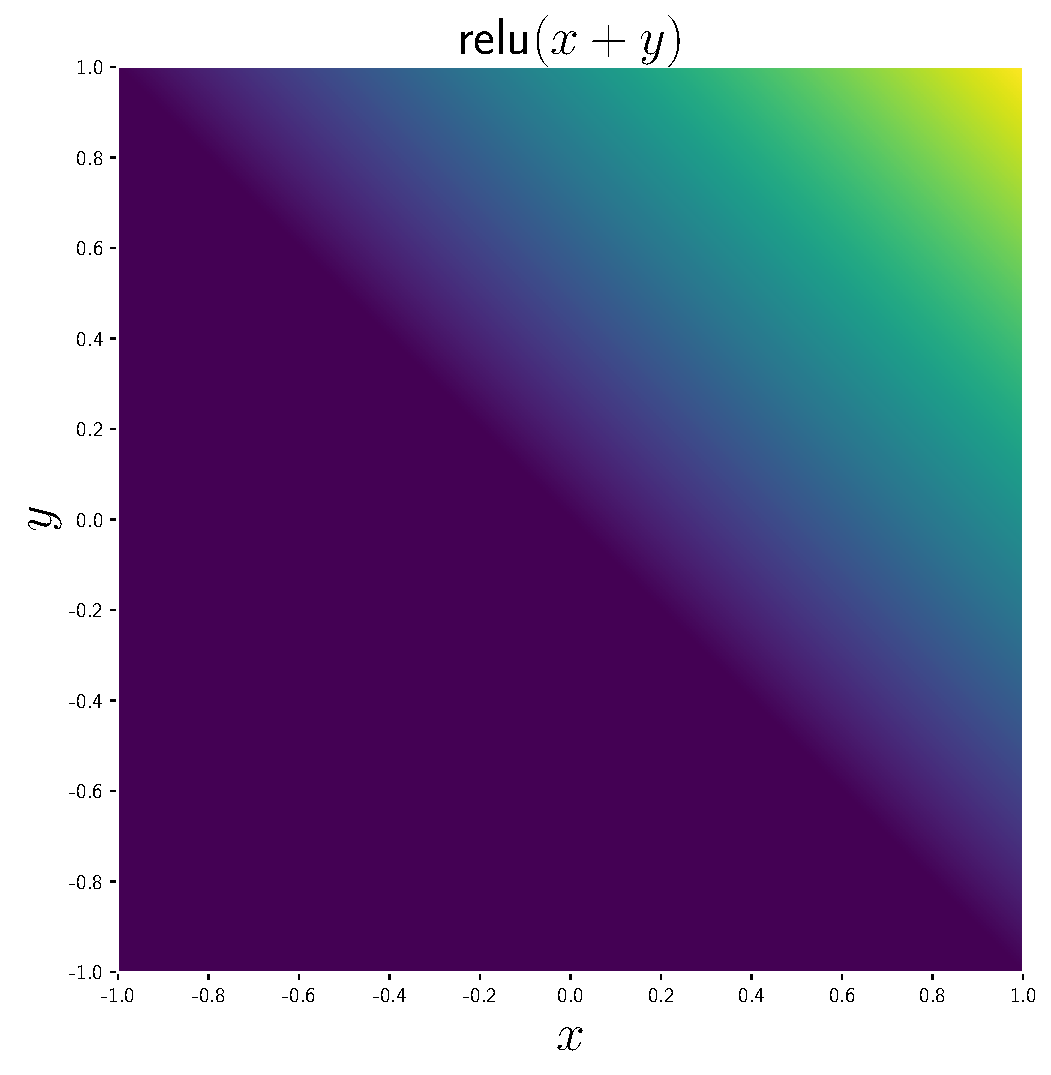
\includegraphics[width=.9\linewidth]{lrc_output}
    \end{subfigure}
    \begin{subfigure}{.45\textwidth}
      \centering
      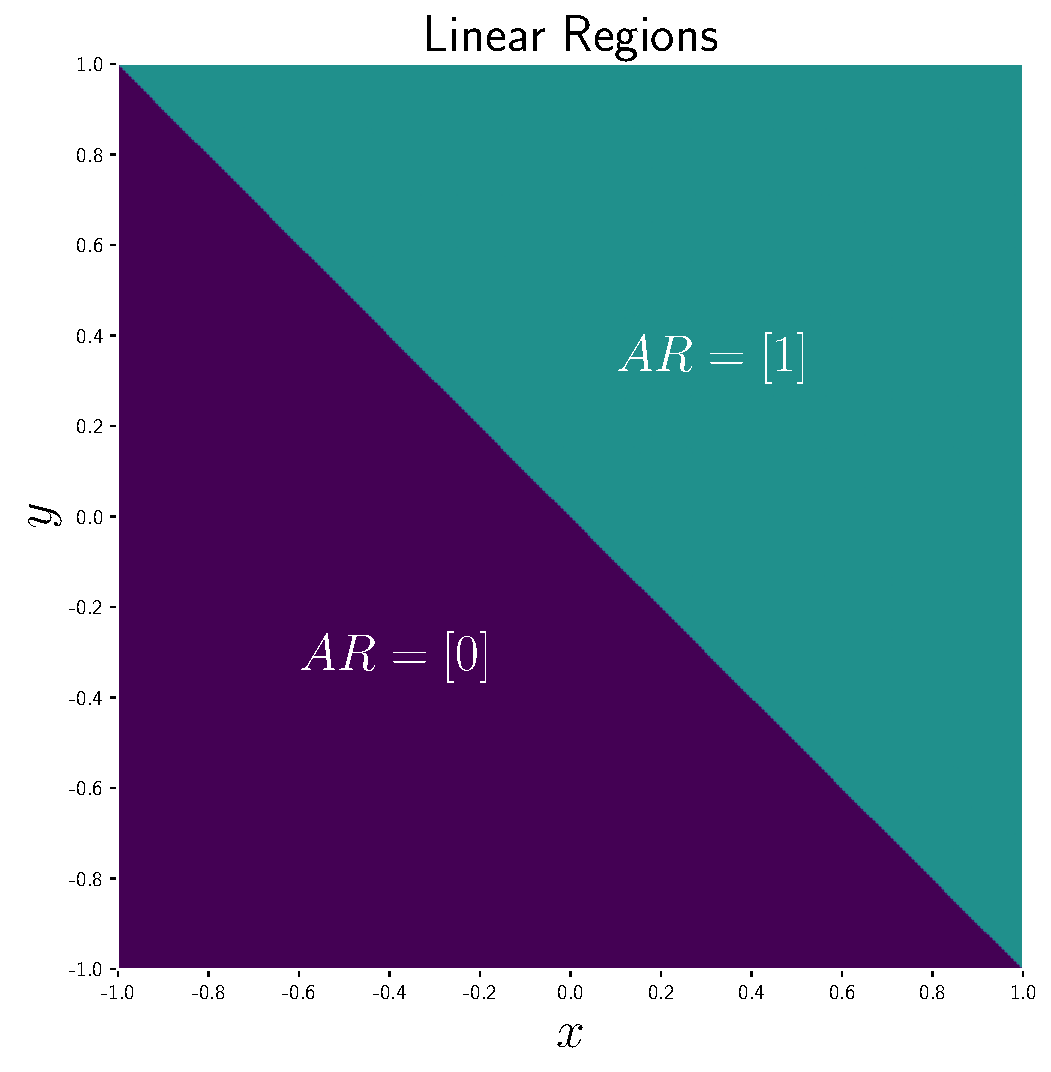
\includegraphics[width=.9\linewidth]{lrc_ars}
    \end{subfigure}
\caption[Activation responses and linear regions of a simple 2D model]{On the left is a simple 2D model $f(x,y) = \text{relu}(x+y)$. The right
shows the two activation responses (AR) and linear regions of that model.}
\label{fig:lrc_2d_example}
\end{figure}
In essence, a ReLU operation folds the input space along some hyperplanar boundary. Multiple ReLU operations perform
compositional, piecewise foldings, further segmenting the input space as shown in Figure~\ref{fig:lrc_complex}.
\begin{figure}[ht]
    \centering
	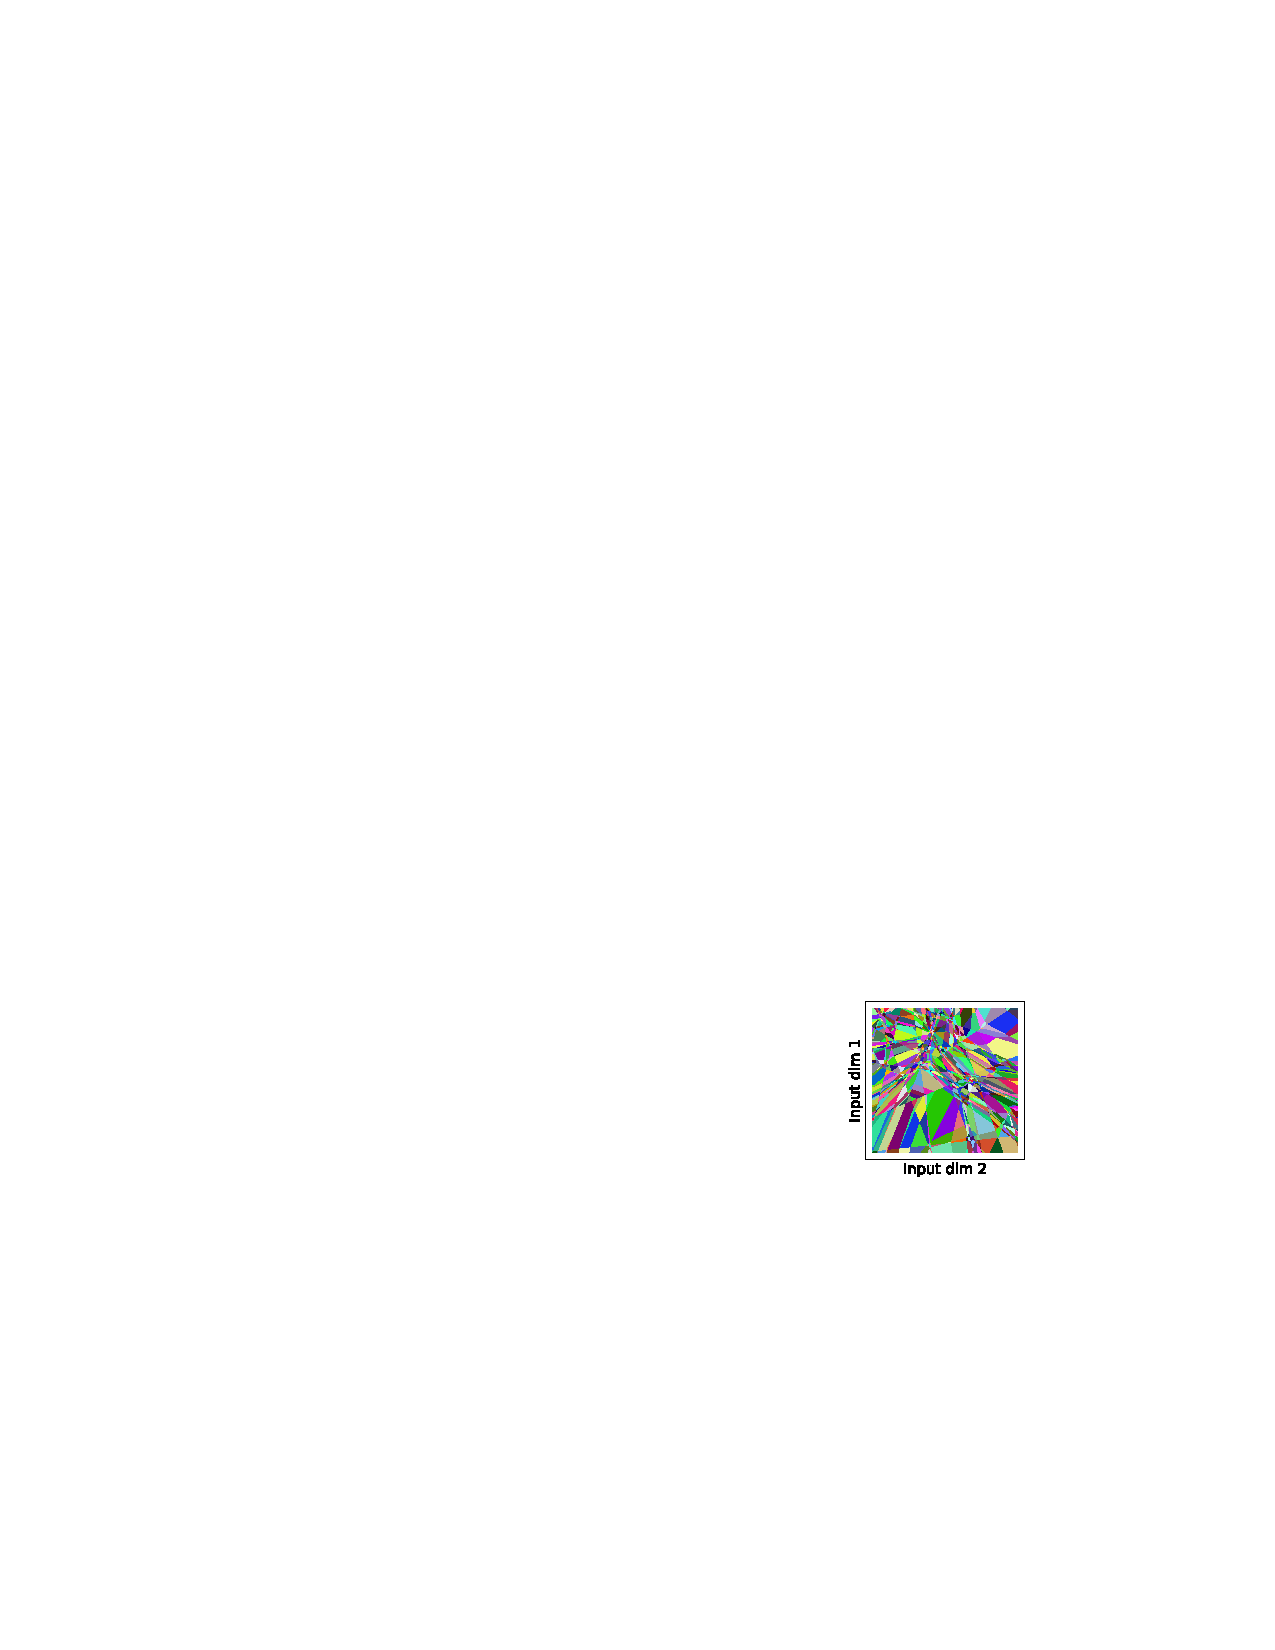
\includegraphics[width=.4\textwidth]{linearregions} \\
	\caption[The linear regions of a more complex model]{The linear regions of a more complex model given a 2-dimensional input, as shown in~\cite{chen2021}.}
    \label{fig:lrc_complex}
\end{figure}

The linear region count therefore measures how efficiently the model performs those piecewise foldings; two models
can have the same number of ReLU operations but perform drastically differently in LRC. For example, one model might
produce exactly orthogonal foldings and therefore have maximal LRC, while another's foldings may be entirely coplanar
and therefore only have a LRC of 2. The crux of all of this is that the more discrete regions of the input space the model
can produce, the more detail it can mathematically distinguish and thus act upon. As such, LRC is used as a proxy
for a model's learning potential. \citeauthor{chen2021} again examine this correlation over NAS-Bench-201, and find a
Kendall-tau correlation of 0.5 as shown in Figure~\ref{fig:lrc_corr}. Examining this plot provides a similar conclusion to that of the NTK analysis: while low LRC can sometimes provide good
performance, high LRC ensures it.

\begin{figure}[ht]
    \centering
	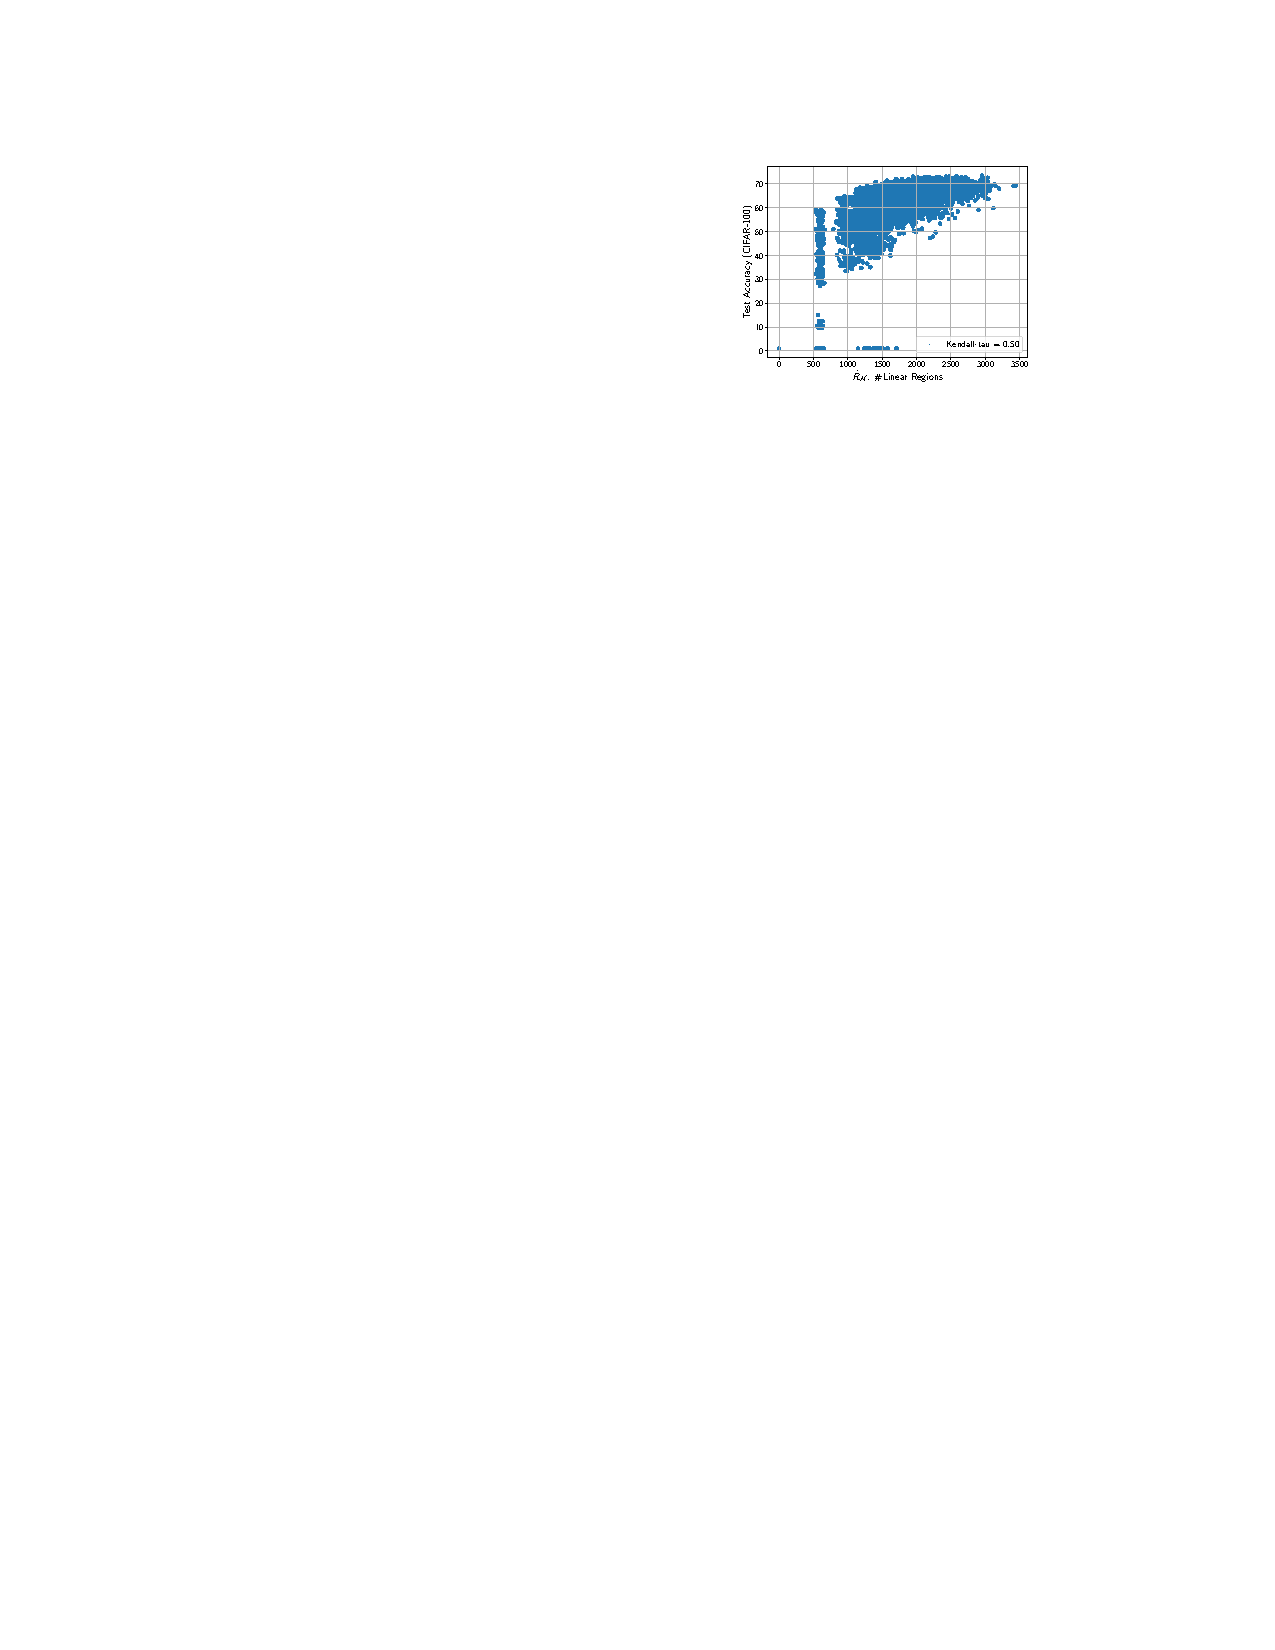
\includegraphics[width=.4\textwidth]{lrc_corr} \\
	\caption[LRC versus model performance on NAS-Bench-201]{LRC versus model performance, NAS-Bench-201 models on CIFAR-100~\citep{chen2021}.}
    \label{fig:lrc_corr}
\end{figure}

To measure LRC in practice, \citeauthor{chen2021} divide the potential inputs of the model into small 3x3 monochromatic regions. A few
thousand of these regions are passed into the model, and the total number of discrete activation responses produced by those
inputs is recorded. This actually performs a subtly different measurement than LRC: rather than absolutely measure LRC,
it measures the number of linear regions produced by that specific subset of inputs. The hope is that the sample is large enough to adequately distinguish differences
in LRC between candidate models, but runs the risk of inaccurately representing the true LRC.
To make a worst-case example, imagine a model that has only $n$ possible linear regions, but those $n$ happen to exactly
align with the sample regions chosen in the LRC sampling. This model would report the maximum possible LRC in the sampling,
and would therefore score equivalently to a perfect model with infinite LRC. This means that \citeauthor{chen2021}'s LRC sampling
cannot meaningfully distinguish the LRC of two models if both models' true LRC equals or exceeds the sample size. While
increasing the sample size could potentially circumvent this issue, this soon becomes prohibitively expensive.
\citeauthor{chen2021} therefore use the same slim models from the NTK measurement to sample LRC from; the slim models have a much
smaller LRC than the full-sized models, one that is sufficiently smaller than the sample size of 3,000 chosen by \citeauthor{chen2021}.
However, this incurs the same approximation problem as NTK, in that it must be assumed that the LRC of the slim models correlates
with the LRC of the full-sized model, again as assumption not touched upon in the original paper and only revealed in the
implementation.

\subsection{Practical Concerns and a Joint NTK-LRC Metric}\label{sect:ntk_practical_concerns}
Caveats about the slim model approximations aside, the practical issue with using LRC or NTK
is that they are both exclusively parameter-value and input dependant:
they provide a meaningful result only when comparing models with identical parameter values over identical inputs.
In order to evaluate models in the search space, \citeauthor{chen2021} use a supernet approach, where any model in the space
can be represented as a subgraph of the supernet. To compare any two models in the space they then create two
identical copies of the supernet, initialize both with
identical parameter values, and then disconnect the irrelevant edges from each supernet. This creates two subgraphs
with identical parameters but different connectivities, and therefore different architectures. This process can
be adapted to compare any arbitrarily large set of models, and this is exactly how \citeauthor{chen2021} evaluate
all the models within the NAS-Bench-201 search space to find the correlations between NTK, LRC, and final test accuracy.

From these results, \citeauthor{chen2021} discover that by adding the descending NTK rank to the ascending LRC rank
of all models\footnote{Here, lower NTKs would provide larger descending ranks, and higher LRCs provide larger ascending
ranks, therefore producing larger combined ranks for models with low NTK and high LRC as compared to other models in the set.}
within the search space provides
a much better correlation with model performance. This makes sense,
if lower NTKs and higher LRCs correlate with better performance, a metric that jointly
rewards low NTK and high LRC would potentially have greater predictive power. The joint NTK-LRC metric
provided a Kendall-Tau correlation of 0.64 with test accuracy which improves upon the -0.42 and 0.5 of NTK and LRC respectively.
The correlation also demonstrates that the slim model approximations used in the calculations of NTK and LRC work well enough,
at least across the search spaces and datasets examined in the paper.

\section{Design}\label{sect:spiderdesign}
\subsection{Models}
Fundamentally, SpiderNet models are near identical in construction to BonsaiNet models. They are cell structured, where each
cell contains edges and nodes. Edges consist of parallel operations, one of each available operation. Each edge contains
operation pruners, to allow deletion of operations from edges. Nodes perform
tensor aggregation, again summation for the same reasons as BonsaiNet. The crucial difference is that each cell has an input
node for each previous cell and the original model input; therefore, the fourth cell has four input nodes
(one for Cell 1, 2, and 3, plus the model input), the third has two, etc. Each cell is
initialized with just its input nodes, one intermediate node, and a single output node. One edge is then placed between
each input and the intermediate node, and then a single edge is placed between the sole intermediate node and the output node.
This configuration is shown in Figure~\ref{fig:spider_multiin_initialization}:
\begin{figure}[ht!]
    \centering
  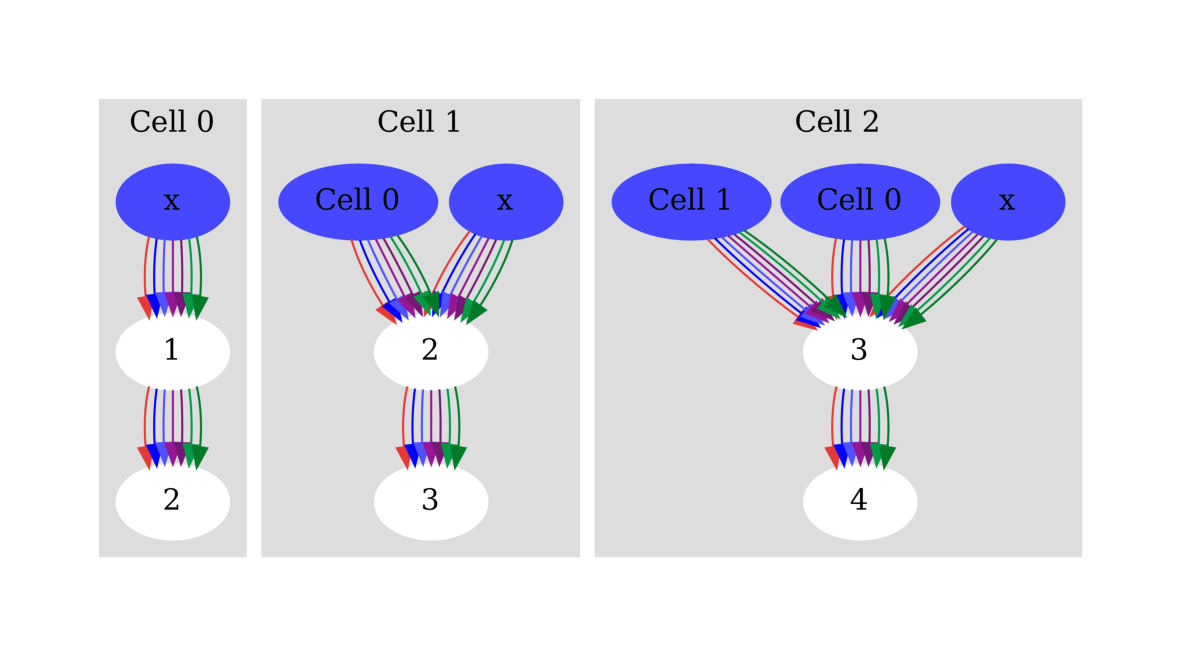
\includegraphics[width=.85\textwidth, trim={0 1.5cm 0 1.5cm}, clip]{graphs/initial_darkerblue}
    \caption[The initial state of a three cell SpiderNet model]{The initial state of a three cell SpiderNet model, with the input nodes marked in blue.}
    \label{fig:spider_multiin_initialization}
\end{figure}

This starting point can be thought of
as a suitably `minimal' starting point as it provides two edges per input: one to the single intermediate and one to the
output. Additionally, the single intermediate has an edge to the output that can combine and synthesize information from the inputs.
Evolutions of this architecture can therefore reinforce the pathways from the input or to strengthen the `mixing' portion of the cell.

\subsection{Mutation}
To accomplish the goal of a dynamically expanding search space, it is first important to define what ``expanding the search space''
actually entails. There are many ways
to define model expansion, and a number of ways of actually designing the mechanism the model would use to accomplish
it. Primarily, to allow the cell's internal connectivity to be evolving and expanding, graph mutations were focused on as the means of expansion.
\added{The term ``mutation'' is chosen here in reflection of~\cite{real2017}'s usage of the term, where it is used to describe graph modification operations
that are applied to candidate models that are similar to ``actions that a human designer may take when improving an architecture.'' The same principle
applies here, in that mutations refer specifically to the graph modification, not necessarily to a stochastic process occurring at random within a gene pool.}
Specifically, the target was a single mutation operation that when
composed with edge deletion via pruners could construct any possible directed acylic graph given some arbitrary starting point.
The operation eventually selected is referred to as a \textit{triangular mutation}, which acts on an arbitrary edge $A\rightarrow B$ that
connects two nodes $A$ and $B$ within a model, adding a third node $C$ and two new edges. These edges are wired such that
for the nodes $A$, $B$, and $C$, one node sends two outputs, one node receives one input and sends one output,
and one node receives two inputs, as shown in Figure~\ref{fig:mutation patterns}.

\begin{figure}[ht!]
\centering
\begin{subfigure}{.43\textwidth}
  \centering
  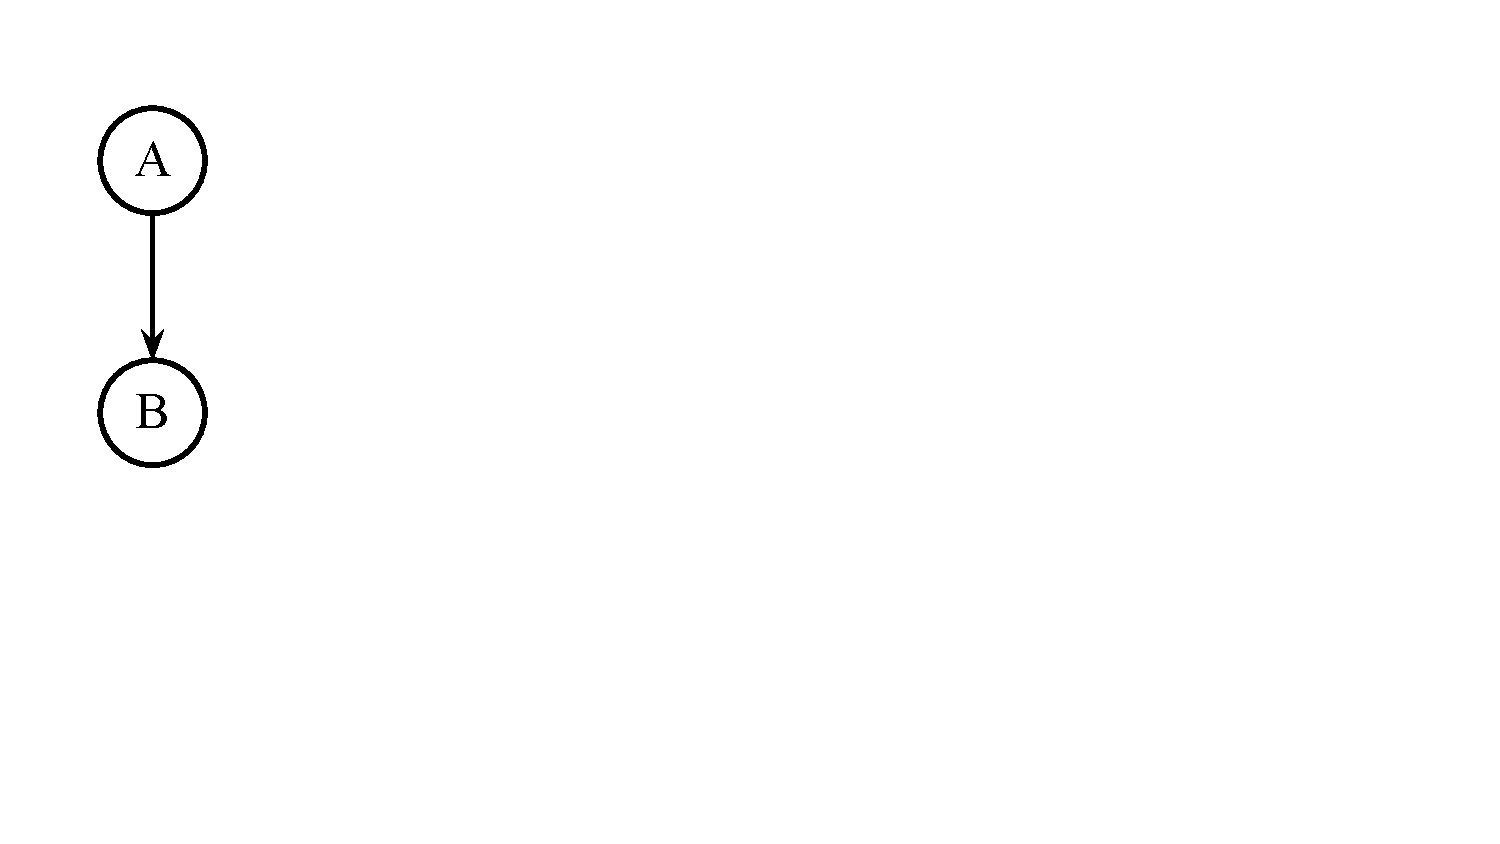
\includegraphics[height=10em]{ab}
  \caption{Original Edge}
\end{subfigure}
\begin{subfigure}{.45\textwidth}
  \centering
  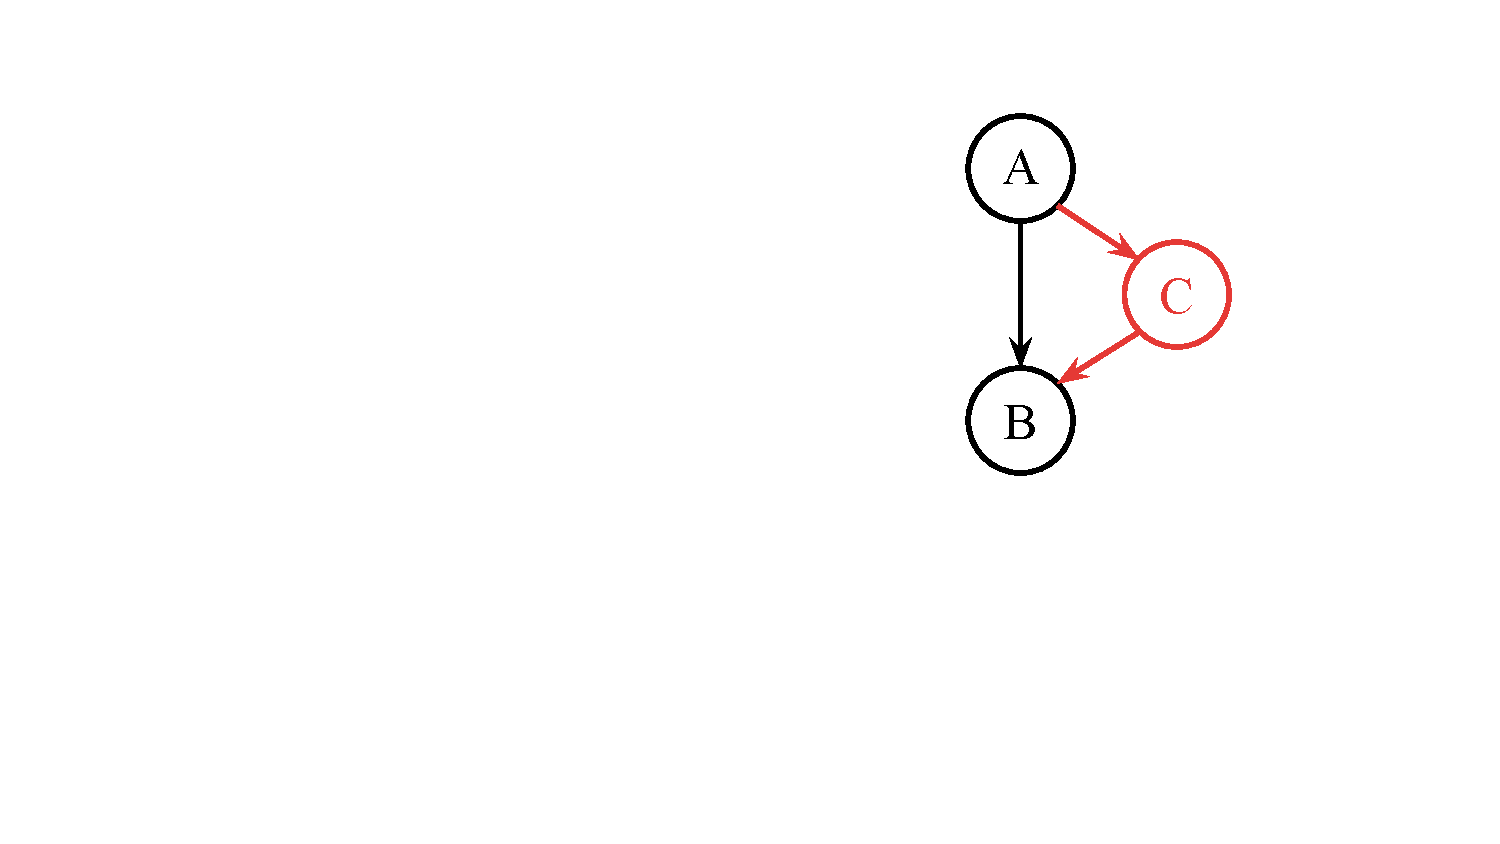
\includegraphics[height=10em]{ab3}
  \caption{Post mutation}
\end{subfigure}%
\caption[The triangular mutation]{The triangular mutation, with new edges and nodes depicted in red.}
\label{fig:mutation patterns}
\end{figure}

\noindent This operation
is composable with edge deletion to create a huge variety of graph patterns, as they all crucially introduce a branching
path into a linear node relationship. This creates a seed for further branching by later
mutations along any of these three edges, which allows a small number of mutations to create immense cellular
complexity.\footnote{The cells split and grow much like the branching propagation of a spider
plant, hence the name SpiderNet and thus continuing the botanical naming scheme started by BonsaiNet.}
For architecture examples of models generated by such triangular mutations, Figure~\ref{fig:spider_rand0_example_main_body}
shows a model after 45 triangular mutations were performed at random. To further see the architectural variance, see more
examples in Appendix~\ref{chapter:appendix_spider}.

\begin{figure}[p]
    \centering
	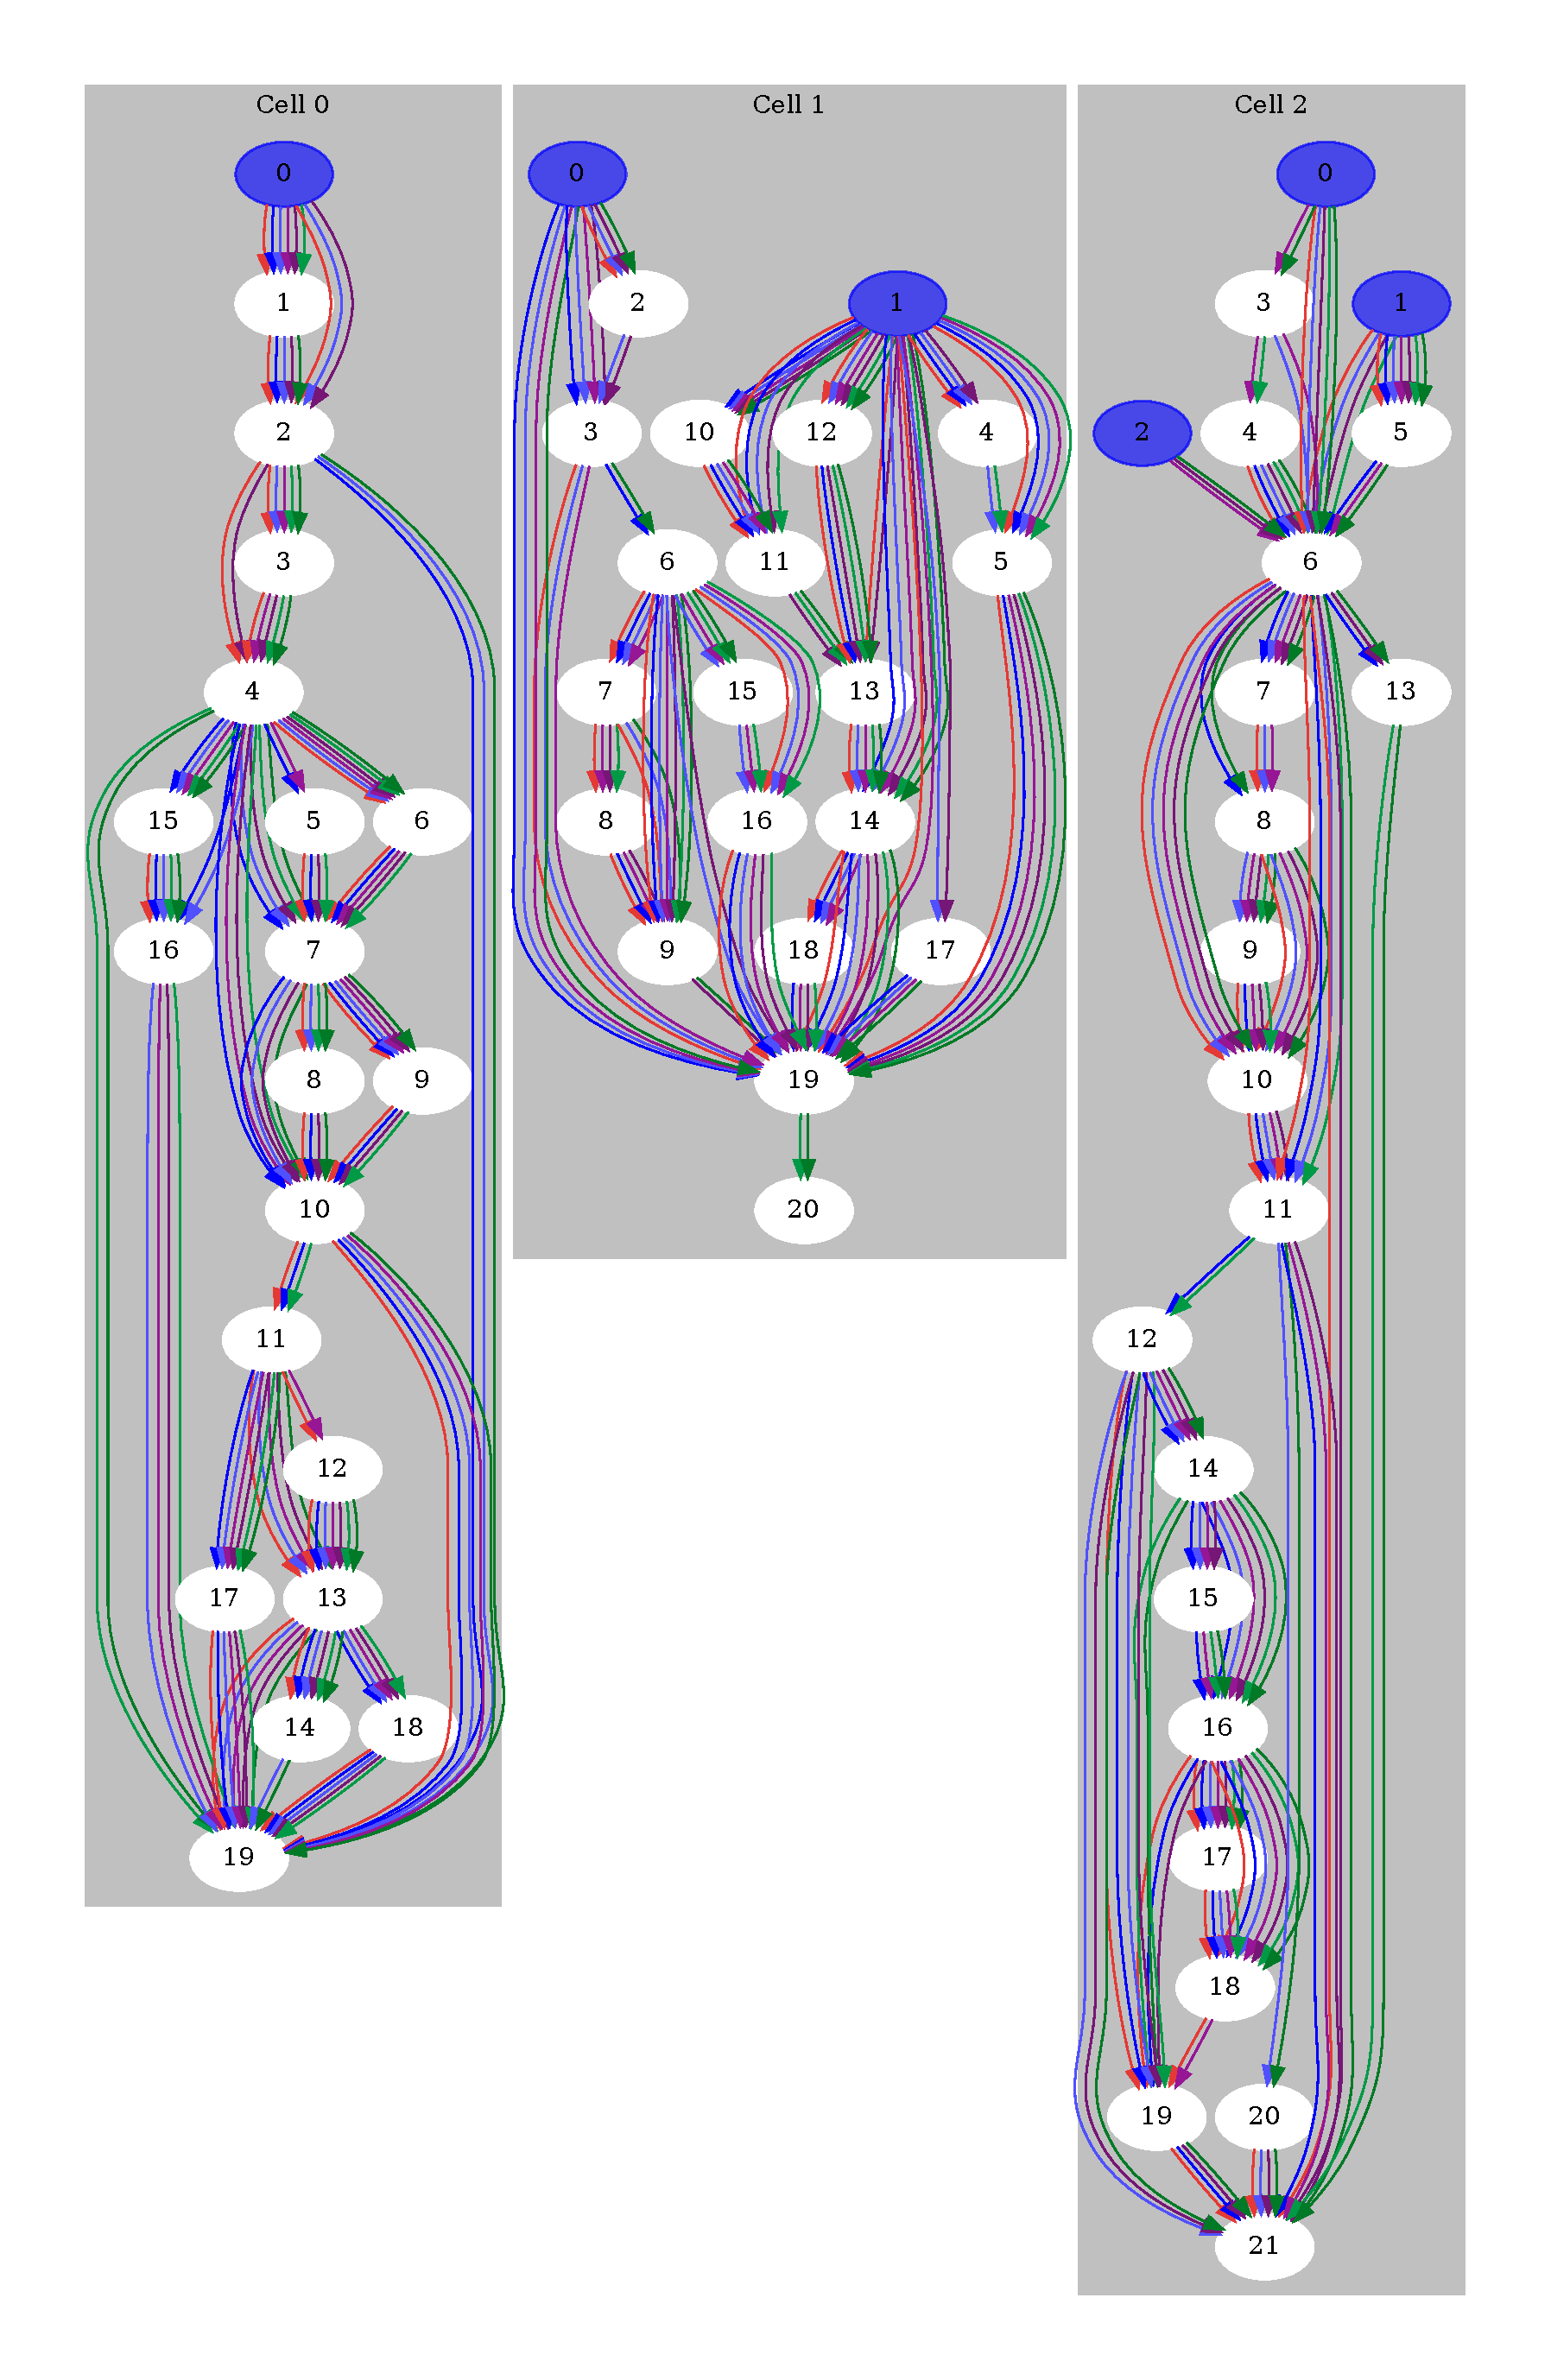
\includegraphics[width=\linewidth, trim={0 1cm 0 1cm}, clip]{graphs/random-2-2} \\
    \caption{A sample SpiderNet model after 45 random mutations. Cellular inputs are shown in blue.}
    \label{fig:spider_rand0_example_main_body}
\end{figure}

A crucial question revolves around what operations the new edges should be initialized with. There are two possible
perspectives to take here. It could be argued that the new edges should be initialized only with operations present
in the original edge; if an edge has deadheaded out a number of operations, it has decided that these operations are
not necessary in this location and thus they should not be placed in the new edges. On the other hand,
new edges might need the opportunity to decide for themselves which operations they need. Considering
that these new edges are not guaranteed to serve the same purpose within the cell, predetermining their initial
operations from a different edge seems premature. For this reason, it seems that this second approach is the better one,
and as such new edges are initialized with all operations from within the operation space. However, this
is based purely on conceptual reasoning, and would require experimental work to fully justify.

\subsection{Mutation Practicalities}\label{sect:spider_mutation_reinit}
Mutations run afoul of the same codependence problem as identified in Section 4.5.3: if new, untrained operations are added
midway through model training, they alter the distributions that downstream operations
are expecting, worsening the model's performance. As such, the new operations were almost
instantly pruned away to restore the connectivity to the model's codependent expectations as best it can,
meaning that the mutation was usually exclusively destructive. To remedy this, the model weights are reinitialized
after each mutation, much like how BonsaiNet resets model weight after pruning cycles. This resets any codependency,
allowing the model to make use of all new operations if it so desires.

\subsection{Selecting Edges to Mutate}
With the edge mutation operation defined, the next step is to identify the mutation criteria; how should the model
select an edge to perform this mutation on? There are three ways to approach this problem; stochastically,
mathematically, or experimentally. Stochastic mutation is easy enough, just randomly select an edge to mutate each time.
If the model does not like the new edges, it can simply prune away the operations and wait for a better mutation next time.
Mathematical mutation would involve defining some metric that is measured over each edge, and then choosing
whichever edge maximizes/minimizes this metric for mutation.

Designing such a metric that determines the most valuable edges to mutate is tricky, but the key insight here is
that the models carry implicit information about the value of their edges via those operations' pruner weights.
There is a variety of summary statistics over these pruner weights, each of which can then be investigated to see if it makes
for a suitable metric for mutation selection. Each potential metric acts over the collective weights of the pruners in the edge from the last
$n$ batches. Therefore, when looking at seven pruners over the last 100 batches, there are 700 data points that the
metric operates over. Four such summary statistics over those batches were identified as candidate metrics:

\begin{itemize}
    \item \textbf{Mean of Pruner Weight}: The mean of the collective weights.
    Higher values of this metric would correspond to edges with more operations that are strongly preserved, while lower
    values imply few operations and strong deadheading.
    \item \textbf{Variance of Pruner Weight}: The variance of the collective weights. High values imply the pruners in this edge are fluctuating significantly, without confidence in whether these
    operations should be preserved or removed. Low values indicate the pruner weights are stable, without much movement
    from batch to batch.
    \item \textbf{Mean of Absolute Pruner Weight}: The mean of the absolute value of the collective weights. High values
    imply that the pruners in the edge have made strong decisions \textit{in either direction} about the operations within,
    while low values indicate that most operations in the edge are close to the decision boundary.
    \item \textbf{Variance of Absolute Pruner Weight}: The variance of the absolute value of the collective weights. High
    values mean that the decisions are varied and fluctuating between batches. Low values again imply consistency in the
    decision making of the pruners, in either direction.
\end{itemize}

In addition to these mathematical metrics, experimental means of determining edge value are also viable as potential
candidates. Here, the importance of each edge in the model is sampled, and this sampled importance is used to inform
mutation. Ideally, the sampling should reflect the independent value of each edge, so that multiple edges can be mutated
simultaneously without worrying about interaction effects. One possible system is Shapley values, specifically
those identified by~\cite{lundberg2017} as described in Section~\ref{sect:spiderbackgroundshap}.

For the purposes of SpiderNet, SHAP is reframed; rather than examine how varying the input features can affect
model output, instead the focus in on how variable model connectivity affects the output, given fixed input. To do this, the edge
connectivity of a SpiderNet model is modeled as a binary vector $\vec{e}$ of length equivalent to the total number of edges in the
model. A 0 at a particular position $i$ indicates the $i$th edge is omitted from the model (corresponding to replacing
that edge with an identity), while a 1 marks the inclusion
of that edge. A subset of the training data is chosen as the fixed input, as therefore the model is transformed
from a function $F(\text{inputs}\;|\;\text{edges})$ to $F(\text{edges}\;|\;\text{inputs})$, that is,
the edge configuration can be varied given a fixed input to see how it alters the output.

To practically do this, each edge in the model graph is assigned an index. When given some binary edge configuration vector
$\bar{e}$ (i.e., the new `inputs' to the model under the new formulation), the edge with index $i$ receives the value $\bar{e}_i$.
If $\bar{e}_i = 1$, the edge performs its usual operation.
Otherwise, it simply performs a zero operation, effectively removing itself from the model. Once the edge configuration
vector inputted to the model has toggled each edge as appropriate, the fixed set of input images is passed through the model
to determine its output.

This model can then be passed into SHAP, which
returns a vector of importances $\vec{\phi}$ for each edge in the model, which indicates how much each edge contributed to the final accuracy
of the model. Large Shapley values indicate that an edge is highly important to a model's performance; its omission
significantly harms the model's accuracy. Small Shapley values on the other hand indicate the opposite, that the edge
can be removed relatively harmlessly. In the extreme, negative Shapley values indicate that an edge is actually detrimental
to model performance, and their removal improves accuracy. While this has obvious utility as a pruning heuristic,
it could also be useful in indicating which edges would benefit most from reinforcement via the triangular mutation.

\subsection{Comparing Metrics}
A convincing argument could be made that any of the above metrics in either direction would be a good mutation target;
for example, you could say that a large mean pruner weight indicates that an edge is highly favored, and thus should
be further strengthened with more edges. Alternatively, a low mean pruner weight could indicate that the current edge is
not valuable, and that it needs more reinforcement to be useful. The SHAP metric is similarly ambiguous; is it better
to add more edges around the most important edges in the model, or is better to reinforce the weaker areas? Given that these arguments can be made for all eight of the
possible metrics, it was best to experimentally test each to determine which produces the best models. To do this,
3 models were tested with identical configuration for each of the 10 metrics (five statistics, with two directions each).
Each model underwent cyclical reinitialization similar to the way BonsaiNet does as described in Section~\ref{sect:breaking codependence}. Here, models were trained until their
first deadhead cycle, then the three edges with the best metric values were chosen for mutation. The model was then reinitialized
and trained for another deadheading cycle, for a total of five cycles. After these five cycles, the model was trained for 64 epochs
to compare their top-end performance. 64 epochs are chosen because comparative performance after 64 epochs between models
is a decent predictor of their final performance rankings. To demonstrate this, Figure~\ref{fig:64epochcorrelations} shows
the Spearman correlation between $n$th epoch accuracy and a final accuracy aggregated over 29 different BonsaiNet and SpiderNet models,
where 64 epochs shows a Spearman correlation to final rank of 0.66.

\begin{figure}[ht]
    \centering
	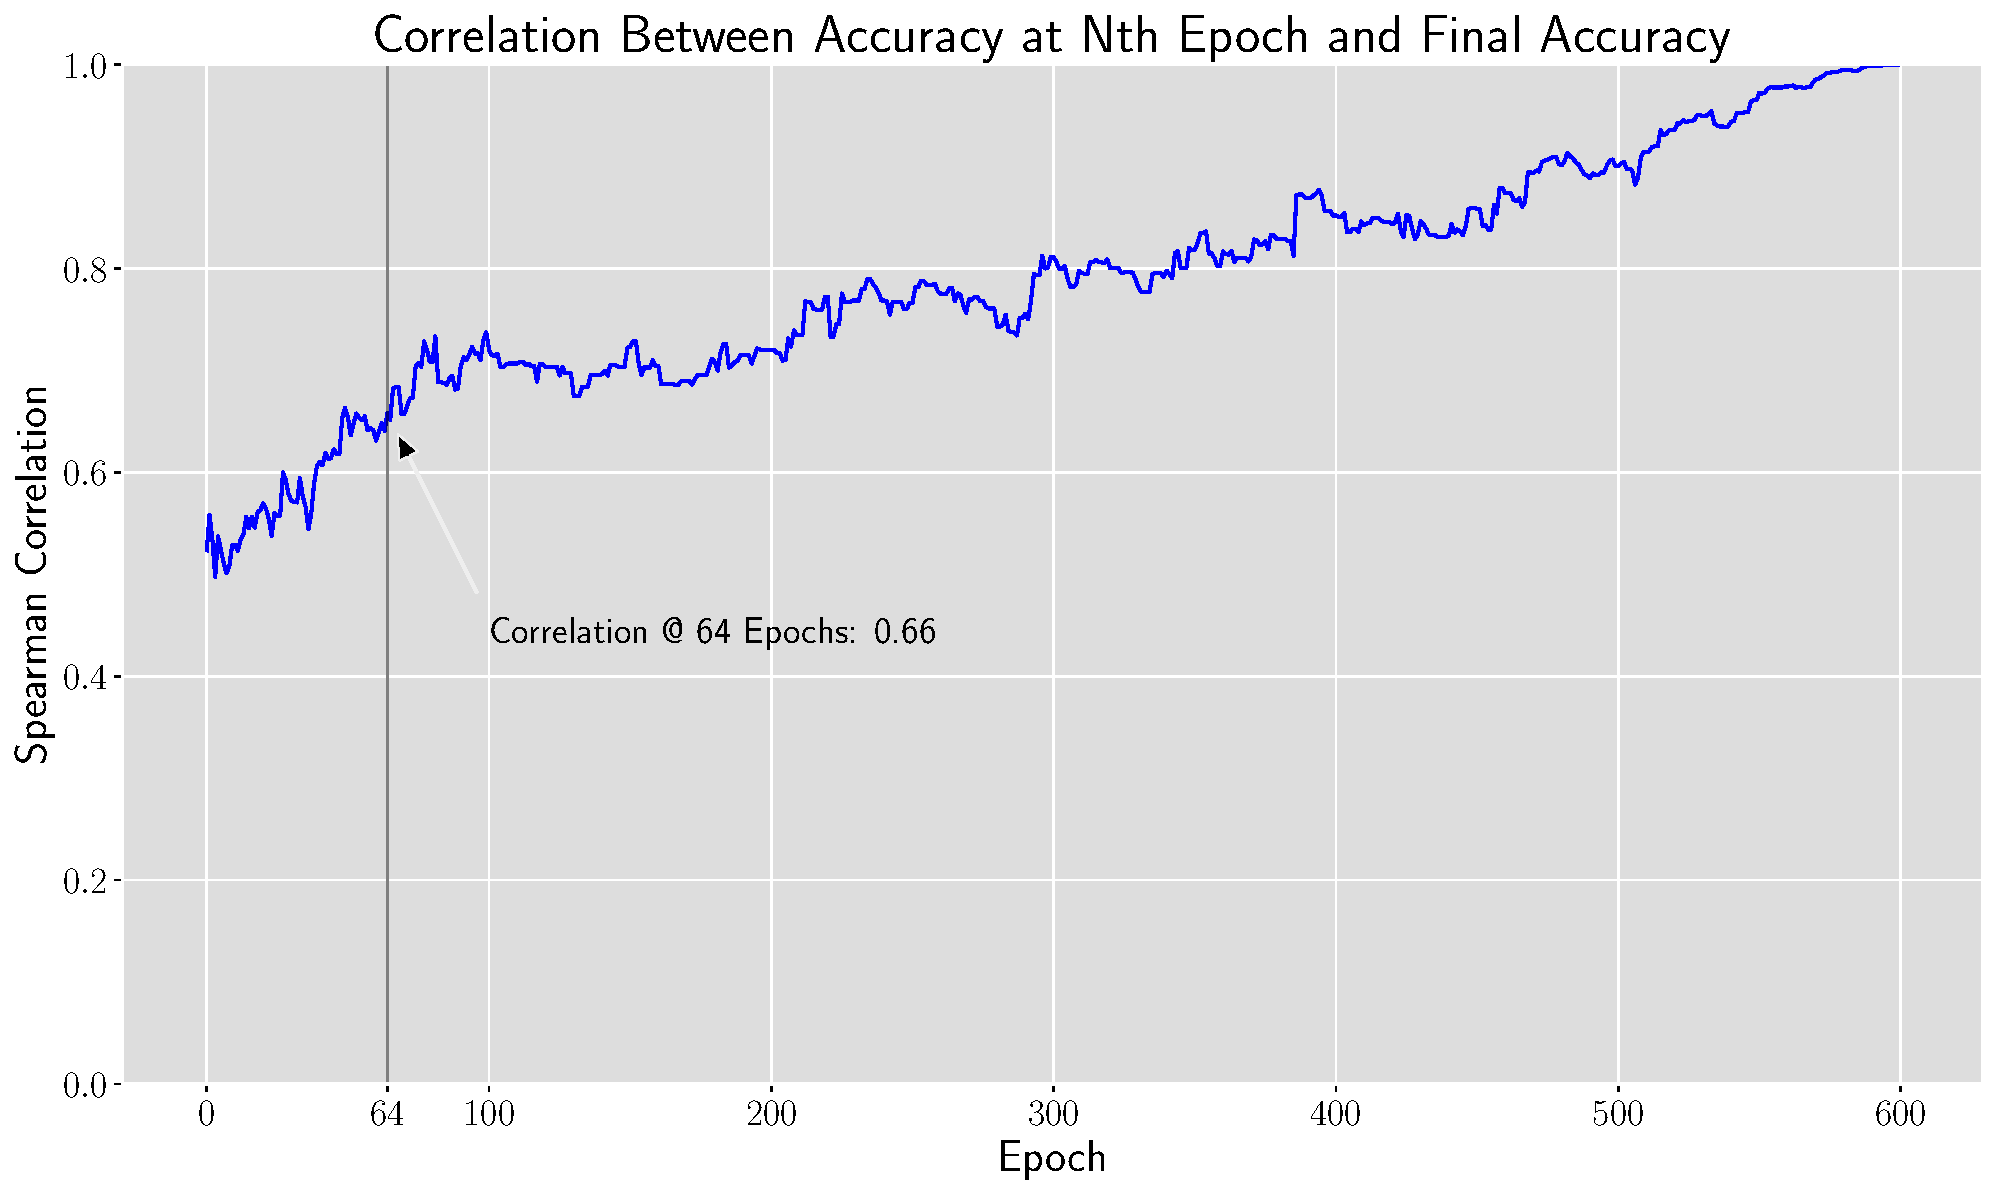
\includegraphics[width=\textwidth]{model_performance_correlations} \\
	\caption[Correlation between models accuracy at 64 epochs and their accuracy at 600 epochs]{Correlation
between accuracy at 64 epochs and their accuracy at 600 epochs over 29 Bonsai and Spider models.}
	\label{fig:64epochcorrelations}
\end{figure}

From this
experiment, the metrics that typically produce the best models can be determined. More importantly, it can be determined how
good a metric is at identifying the best mutation candidate by comparing it against its opposite metric; if choosing
edges that have the maximum values of some metric identifies the best possible operations to mutate,
choosing the minimum valued edges should be the worst possible. Therefore, the aim is to find a metric which produces
a large performance gap between its minimum and maximum case. While a metric not having a clear difference between
its maximum and minimum case does not imply it is poor at distinguishing good and bad mutation candidates (as it
could simply be indicative of a non-linear or bell-curved ranking; perhaps the maximum and minimum is the worst and the
most central value is optimal), choosing a metric with a linear ranking is simplest conceptually and mathematically. These
differences between minimum selection and maximum selection are shown in Figure~\ref{fig:mutation_metrics_full_train},
which represents the comparative \textit{search} performance of each metric.

\begin{figure}[ht]
    \centering
	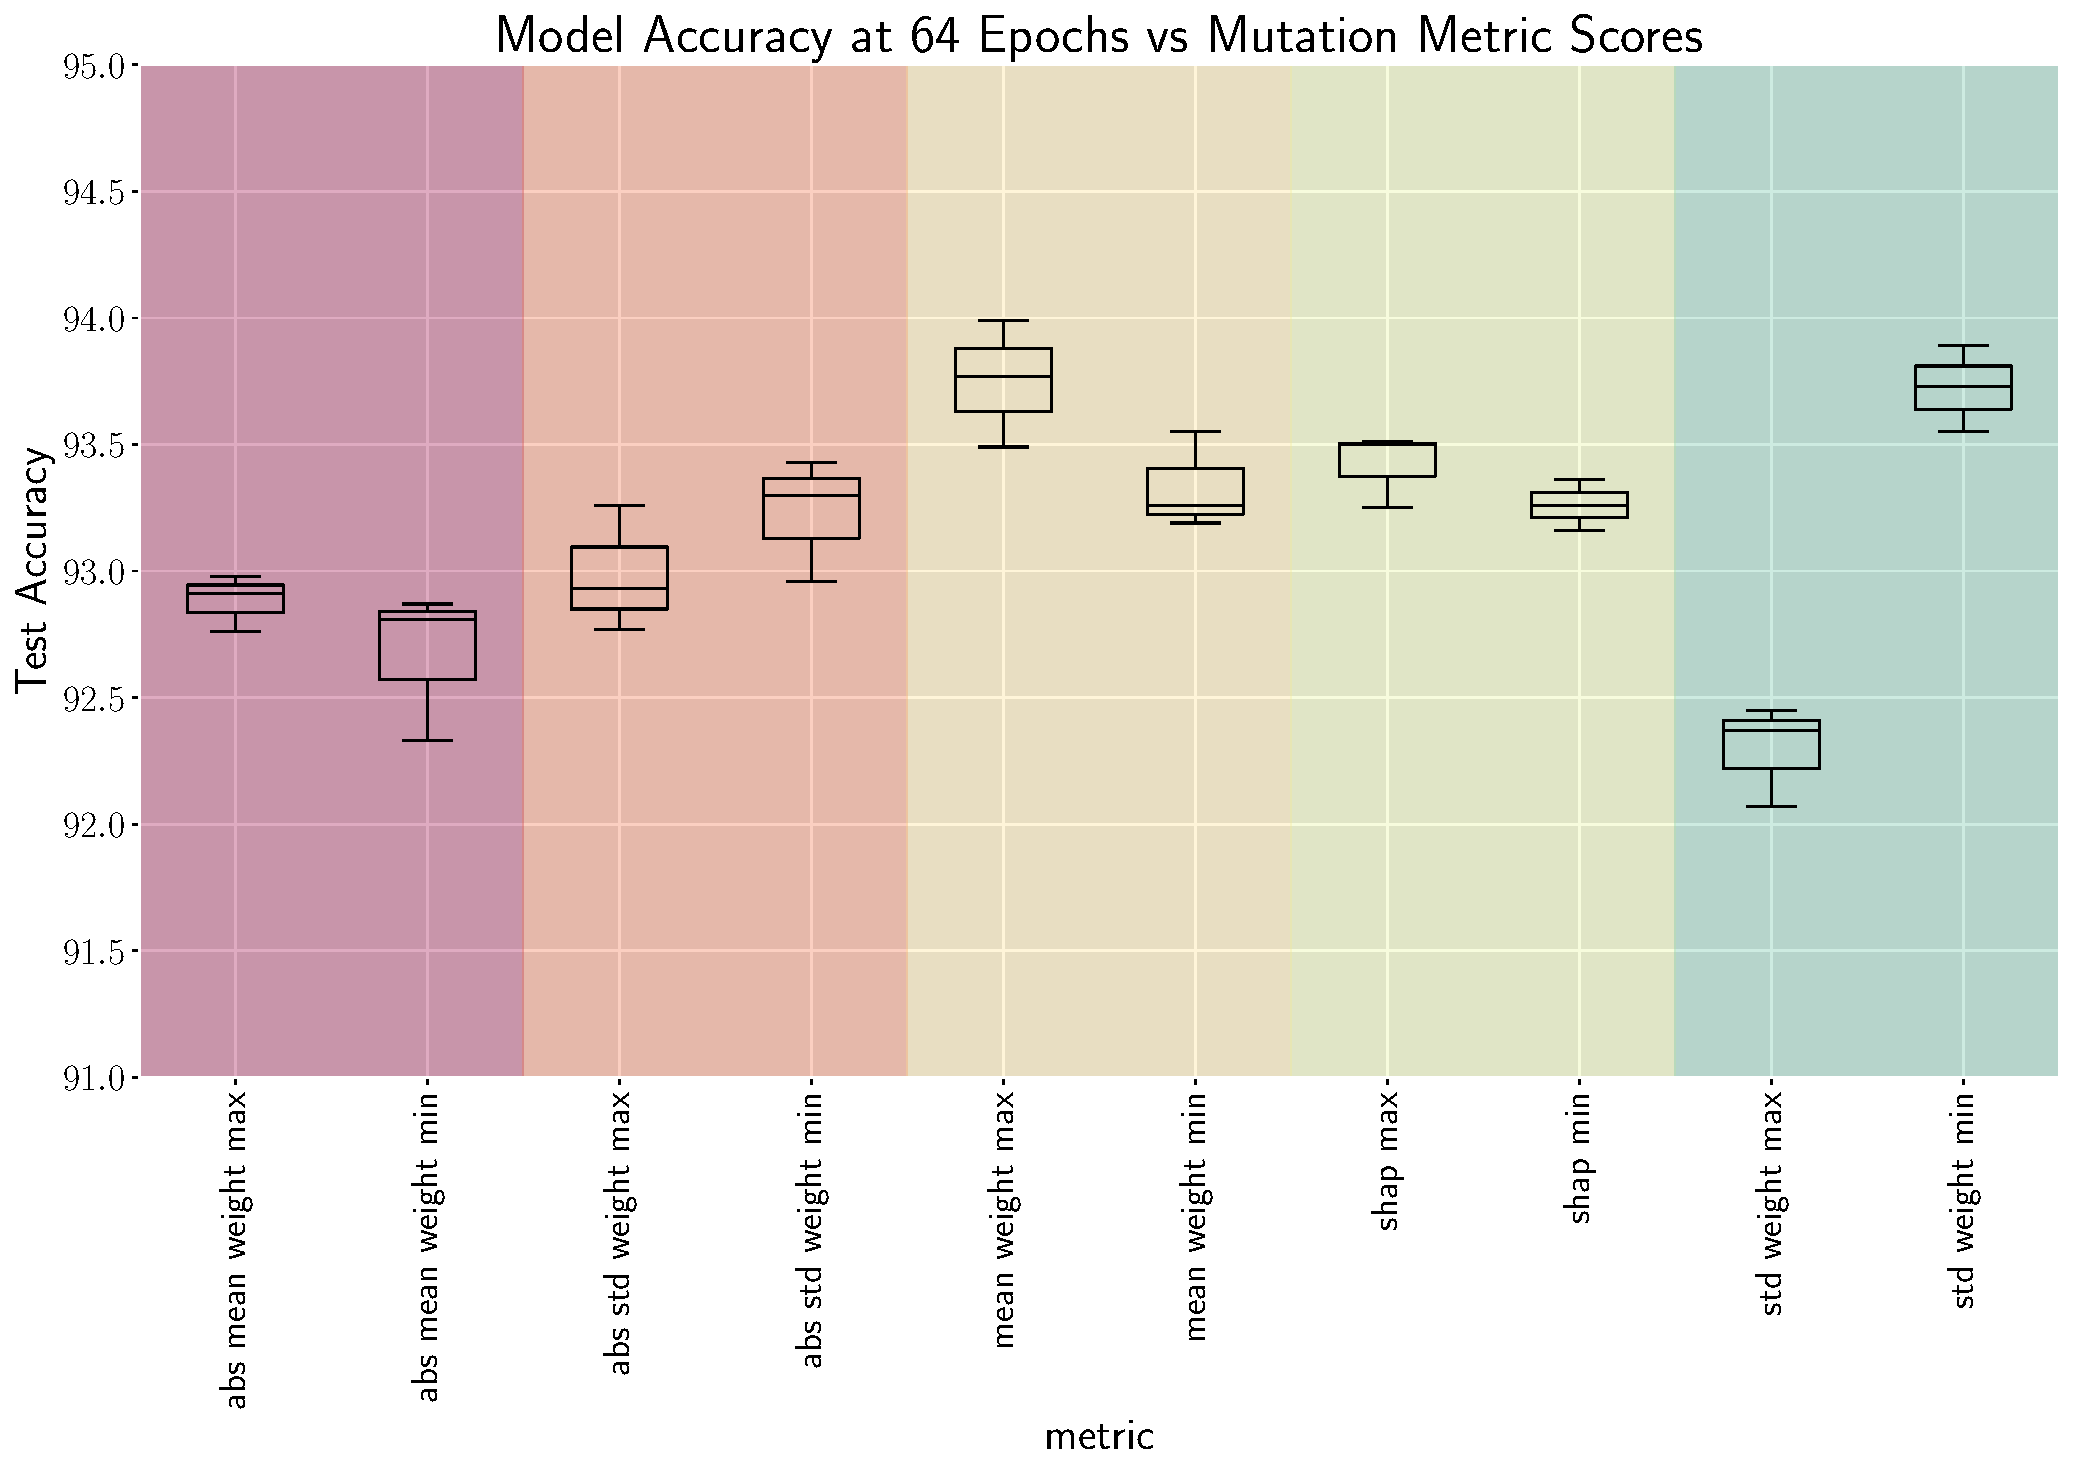
\includegraphics[width=\textwidth]{accuracy_after_64_epoch} \\
	\caption[Performance after five mutation cycles and 64 epochs of training for each of the 10 mutation metrics]{Performance after five mutation cycles and 64 epochs of training for each of the 10 mutation metrics, with
    the results of three separate models shown in each case. This shows each metric's relative ability to search for
    architectures, that is, their how well each metric mutates edges based on their \textit{future} effect on performance.}
	\label{fig:mutation_metrics_full_train}
\end{figure}

A few things stand out from these results. First, the best overall models were produced by mutating the edges with the
maximum mean or minimum standard deviation\footnote{This metric is also referred to as maximum/minimum variance throughout this thesis.}
of pruner weights. This indicates that edges with many operations preserved
confidently or pruners that are steadfast in their weights are the best to mutate. More interestingly, notice that
while minimum variance models produce some of the best models, the maximum variance models produce
three of the four worst models in the entire experiment. This is indicative of that ideal linear ranking that was hoped
for, which indicates meaningful difference between the minimum and maximum values of the pruner weight variance metric.

An alternative perspective to take is to identify which metrics produce the most consistent improvement to models
cycle-on-cycle. This therefore looks at how a metric might affect a model's performance in the directly subsequent cycle,
thus evaluating short-term performance changes versus the lifetime changes evaluated in
Figure~\ref{fig:mutation_metrics_full_train}. In essence, the previous analysis gave each metric's ability to select edges
that \textit{will} limit model performance, whereas now it will be each metric's abilty to identify edges that \textit{have already}
hindered performance. To view this, the accuracy of each model after each mutation cycle and training period is plotted for
each of the 10 metrics in Figure~\ref{fig:mutation_metrics_cycles}, which represents the comparative
\textit{tuning} performance of each metric.

\begin{figure}[ht!]
    \centering
	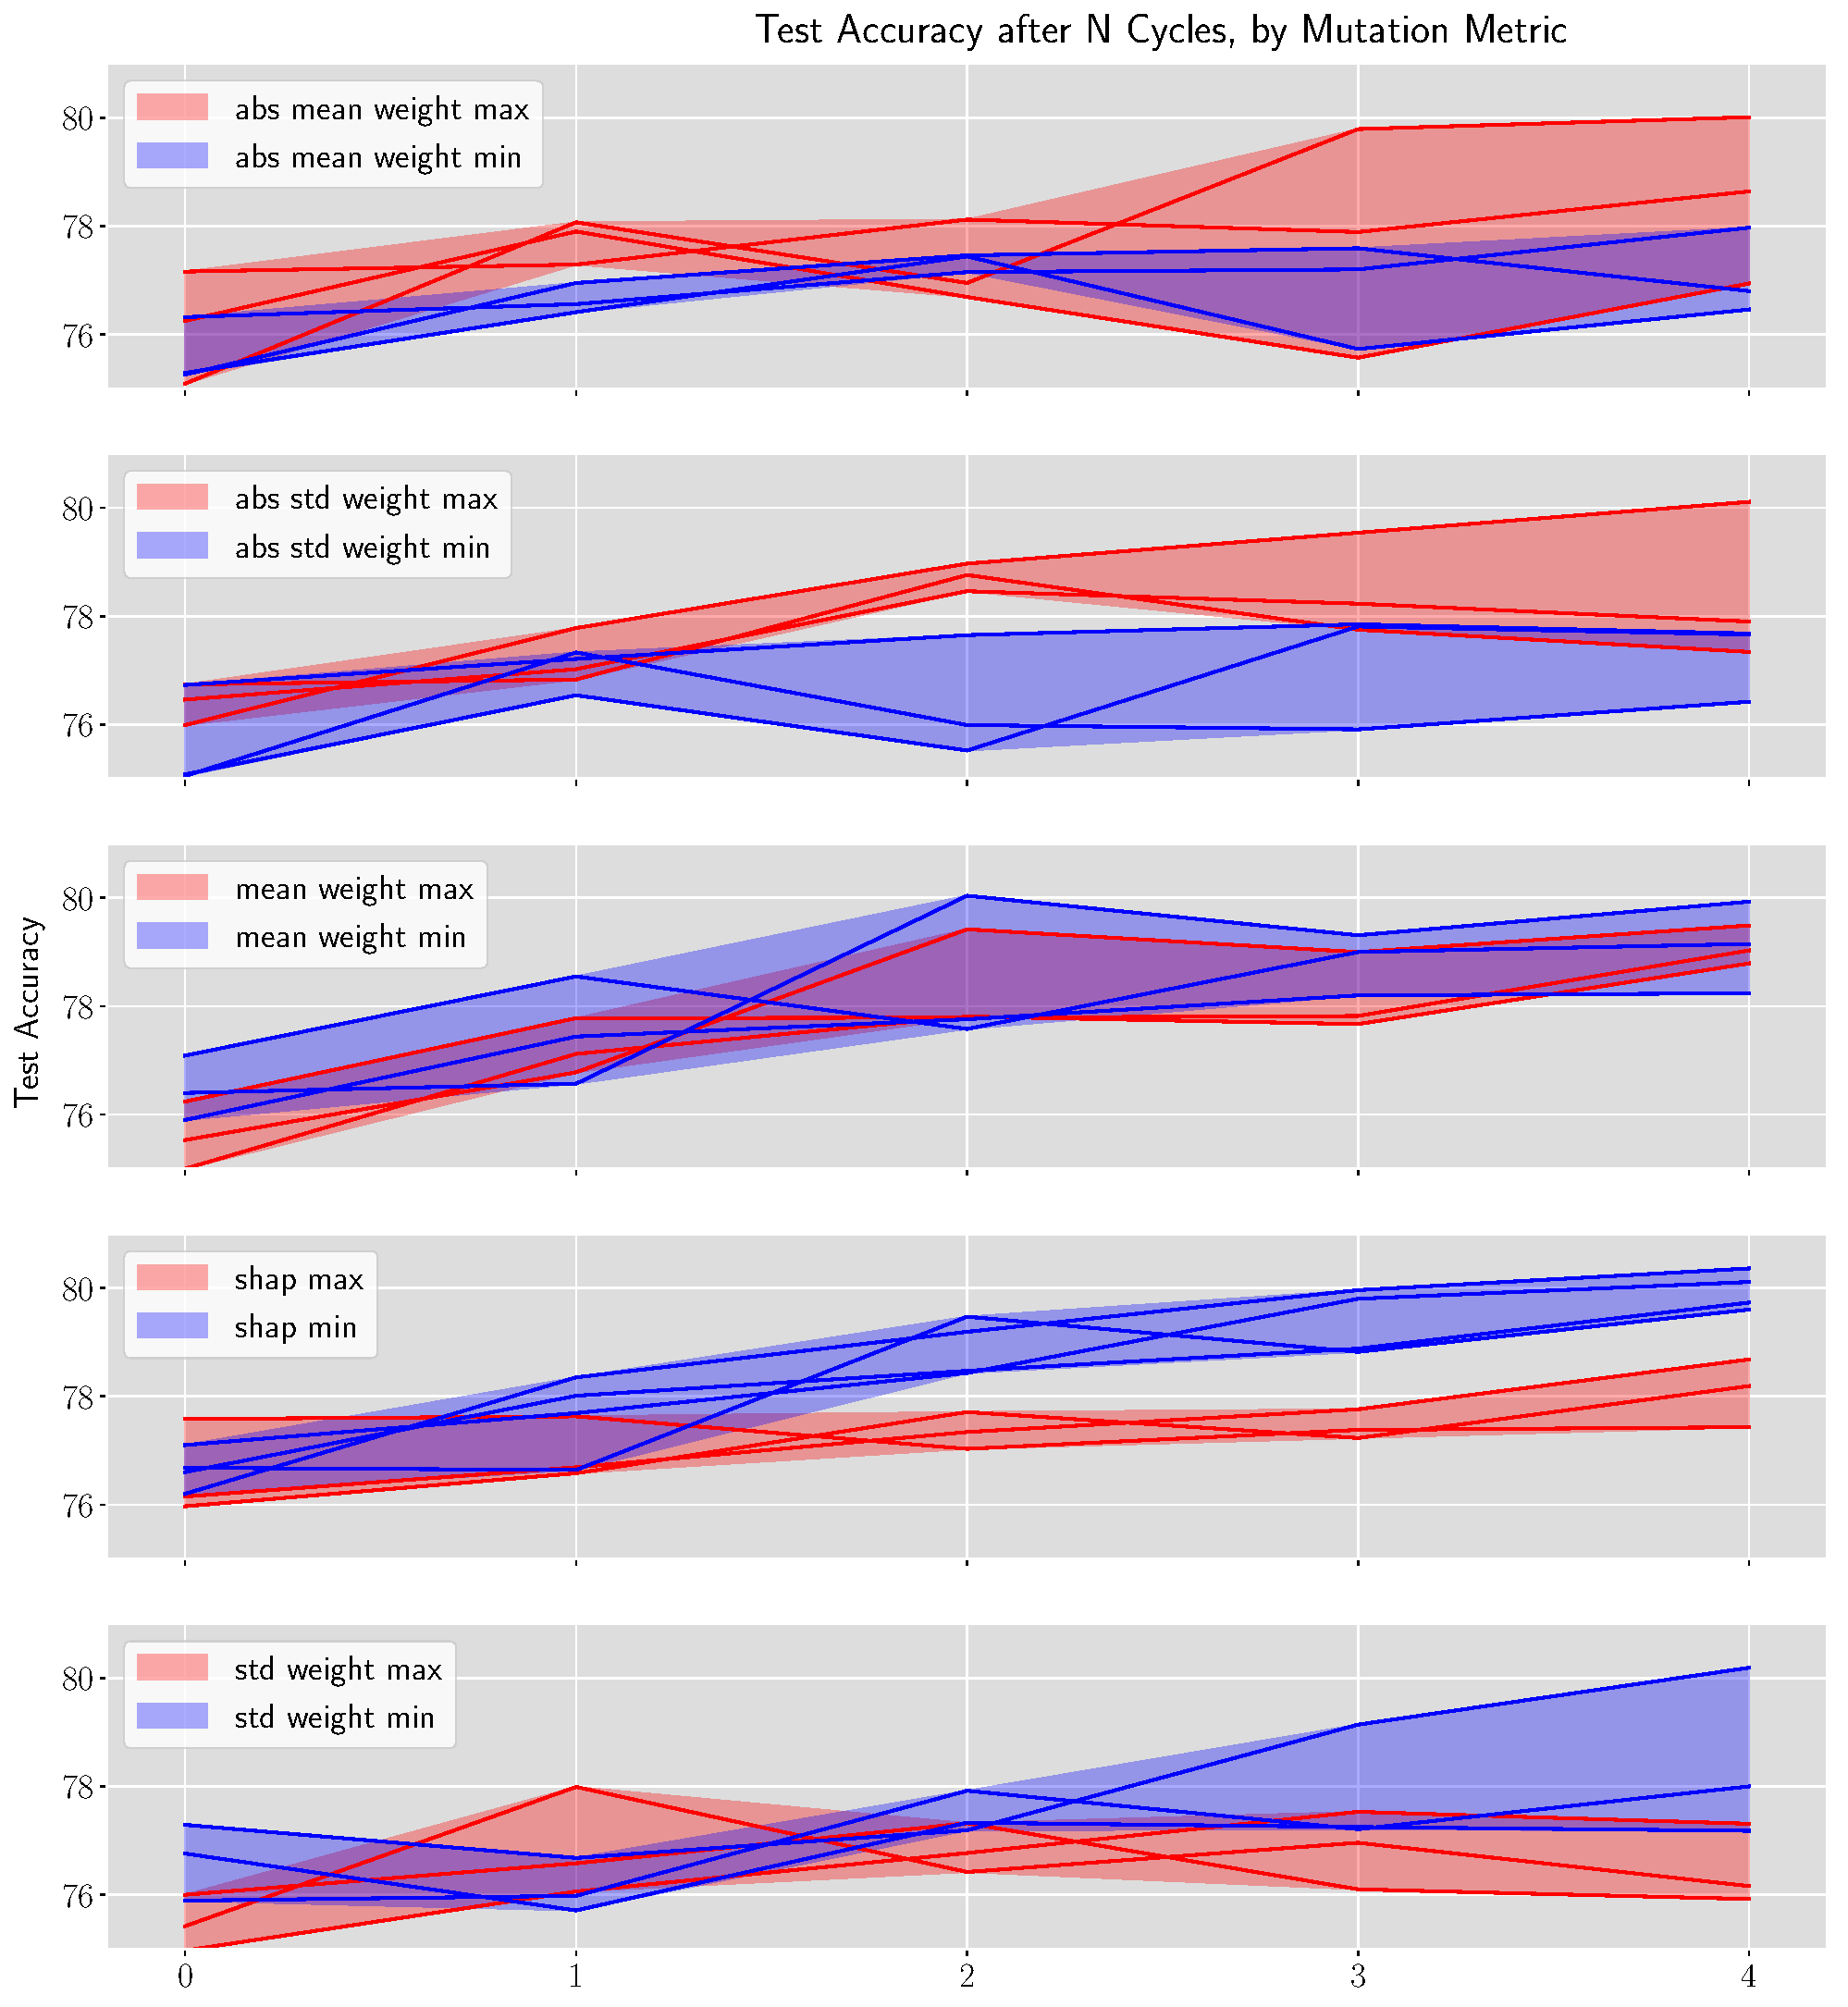
\includegraphics[width=\textwidth]{accuracy_after_n_cycles} \\
	\caption[Performance at the end of each mutation cycle for each of the 10 mutation metrics]{Performance at the end of each mutation cycle for each of the 10 mutation metrics, with the performances
    of each of the three models overlaid. This indicates each metric's relative ability to tune architectures, that is,
    how well each metric mutates edges based on their \textit{extant} effect on performance.}
	\label{fig:mutation_metrics_cycles}
\end{figure}

There are a few key insights within this plot. Notably, most metrics trend upward cycle-on-cycle, with the exception
perhaps being maximum standard deviation. However, this is likely just due to the model size increasing cycle-on-cycle,
as each post-cycle mutation adds a significant number of differentiable parameters to each model. Another interesting
thing to note is that the minimum and maximum SHAP metrics are the only two that produce consistently ranked models;
all minimum SHAP models perform better than all maximum SHAP models from the second cycle onwards. This is in contrast
to its relatively poor, non-discriminative performance in the search case. This indicates that the minimum SHAP model
is excellent at identifying edges that have already hindered performance, but that neither metric is particularly
able to make accurate predictions about the future performance impacts of edges. This result does make intuitive sense
in hindsight; the SHAP metric produces a score that describes each edge's exact influence on the current model accuracy,
but has no ability to discern future accuracy.

Of these candidates, minimum variance seems most promising, given its strong performance
in Figure~\ref{fig:mutation_metrics_full_train}. Since it produces the largest and clearest
distinction between maximum and minimum values of the metric after the fixed mutation cycles, it appears to
prioritize beneficial mutations. However, there is still one more candidate to consider, which will be looked
at in the following section.

\section{Train-Free Mutations}\label{sect:spider_tf_mutations}
One final approach that can be taken to determine optimal mutations is to look at a train-free metric like NTK-LRC.
Such a metric would allow for the entire model to be mutated immediately, which would
drastically reduce search cost.

\subsection{Searching via Joint NTK-LRC Metric} \label{sect:ntk_metric}
While in theory the NTK-LRC metric allows for every candidate in the search space to be evaluated `for-free' in terms of model
training, the actual computation of the two metrics still comes with a non-trivial computation cost. For reference, calculating
the NTK-LRC of a model comparable in size to those produced by BonsaiNet takes around a minute. Therefore, for larger
search spaces the entirety of the space still cannot be fully enumerated, and must be traversed in some intelligent manner.
In the case of the DARTS space, \cite{chen2021} create a tournament selection~\citep{miller1995} algorithm to find good architectures.
Here, a `champion' model $M$ is compared against a set of challenger models $\mathcal{M}$, each $M'\in\mathcal{M}$ created
by removing one operation at random from $M$. The model $M'\in\mathcal{M}$ with the best joint NTK-LRC is then chosen as
the next champion, and the process repeats until a satisfactory model is found. In essence, this is a train-free method
of iteratively pruning a supernet to find an optimal subnet, and from this approach \citeauthor{chen2021} find state-of-the-art
results comparable to those found by DARTS.

However, as has been discussed at length in thesis, any random model within the DARTS space has the potential to provide
state-of-the-art results. How might this method fare in an unbound search space like that of SpiderNet? To examine this,
\citeauthor{chen2021}'s tournament selection can be adopted to measure the quality of potential mutations. Given some
model $M$, the set of all models $\mathcal{M}$ that are one mutation away from M is enumerated. The NTK and LRC of
each mutated model $M'$ is compared against the original unmutated model $M$, and the model $M' \in \mathcal{M}$ that
maximizes the combined NTK-descending and LRC-ascending ranks is selected, if such a model exists. This process can then
be repeated a number of times, in theory improving the quality of the model after each cycle.

The practical caveat to this approach is the aforementioned cost of evaluating NTK and LRC; if each takes around a
minute to evaluate each potential mutation, exhaustively comparing every possible mutation can take around an hour for
larger models. This means that the process of finding a single mutation can take an hour, which over the course of many
mutation cycles gets prohibitively expensive. To avoid this, mutation candidates are instead sampled at random, and after
a certain configurable number of `good' mutations are found (i.e., ones that do not increase NTK and do not decrease LRC,
therefore producing a model that is at worst equivalent to the original model) the sampling ends. Of these found
good mutations, the best one in terms of NTK-LRC is performed on the model. This drastically reduces the number
of NTK-LRC computations necessary to find a good mutation, other than in the worst-case scenario where every mutation candidate
is bad. While this does generally speed up mutation time significantly, it does
come at the potential expense of mutation quality; when the candidates are fully-enumerated, the absolute best mutation can be
chosen each time. When sampling, only a relatively good one is guaranteed.

With this, NTK-LRC can now be used as a mutation metric, and Algorithm~\ref{alg:ntklrc} describes how the NTK-LRC mutation
metric selects candidate edges for mutation.

\begin{algorithm}[ht]
\SetAlgoLined
\SetKwInOut{Input}{Input}
\SetKwInOut{Output}{Output}
\Input{Some model $M$ and sample size $n_{good}$}
Let $s(x)$ refer to the VRAM size of some component $x$ as per Algorithm~\ref{alg:revised_operation_sizing}\;
Let $s_{max}$ be the maximum permitted VRAM allocation\;
\lnl{ntk:slim} Create $S$, the slim model of $M$\;
Let $\mathcal{E}=\varnothing$\;
\lnl{ntk:loop}\For{\upshape edge $e$ in $M$, selected in random order}{
    \lnl{ntk:copying} Let $S'$ be an exact copy of $S$\;
    \lnl{ntk:mutate} Mutate $e$ in $S'$, thus creating two new edges $e'$ and $e''$\;
    \lnl{ntk:copy_again} Create an identical copy of $S'$ and label the two $S_{on}'$ and $S_{off}'$\;
    \lnl{ntk:disconnect} Within $S_{off}$, disconnect $e'$ and $e''$\;
    \lnl{ntk:compute} Compute NTK and LRC for $S_{off}$ and $S_{on}$\;
    \lnl{ntk:add}\If{\upshape NTK$_{on}$ $\le$ NTK$_{off}$ and LRC$_{on}$ $\ge$ LRC$_{off}$}{
        Add $e$ into the set of good mutation candidates $\mathcal{E}$\;
    }
    \lnl{ntk:break} \If{$|\mathcal{E}| \ge n_{good}$}{
        break\;
    }
}
\If{$|\mathcal{E}| > 0$}{
    \lnl{ntk:findbest} Let $e^*$ be the candidate mutation with best joint NTK-LRC in $\mathcal{E}$\;
    \lnl{ntk:iffits}\If{$s(M) + 2s(e^*) < s_{max}$}{
        \Output{$e^*$}
    }
}
\Output{$\varnothing$}
\caption{NTK-LRC Mutation Selection}
\label{alg:ntklrc}
\end{algorithm}

The NTK-LRC algorithm works by first creating a slim model $S$ of our SpiderNet model $M$ in line~\ref{ntk:slim}, as described in
Section~\ref{sect:ntk_intro} and \cite{chen2021}. This is done by initializing an exact copy of the SpiderNet model,
and then reducing the channel count of each operation down to 1. Next, line~\ref{ntk:loop} selects edges at random from the model
as potential mutation candidates. Before trialling the mutation of some selected edge $e$, line~\ref{ntk:copying} creates
an identical copy $S'$ of our slim model $S$; all trial mutations are performed on the copy, thus keeping
the original slim model $S$ as an unmodified template that can be used again. Edge $e$ is then mutated within $S'$ in line~\ref{ntk:mutate},
thus creating two new edges $e'$ and $e''$ as per the rules of triangular mutation. Next, a copy of the mutated $S'$ is made in
line~\ref{ntk:copy_again}. This creates two identical mutated models, the original $S'$ and the copy, which
are then labeled as $S_{on}'$ and $S_{off}'$. Within $S_{off}'$, the new edges $e'$ and $e''$ created by the mutation are
disconnected (simply by multiplying their outputs by 0); this means that $S_{off}'$ is now mathematically identical
to the original unmutated model $S$, but physically has the same parameters as $S_{on}'$. See Figure~\ref{fig:ntk_s_models}
for a simplified visualization of $S$, $S_{on}'$, and $S_{off}'$ at this stage of the algorithm.
\begin{figure}[ht!]
\centering
\begin{subfigure}{.3\textwidth}
  \centering
  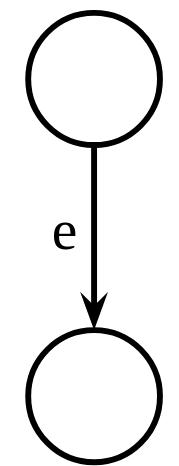
\includegraphics[height=10em]{s}
  \caption{$S$}
\end{subfigure}
\begin{subfigure}{.3\textwidth}
  \centering
  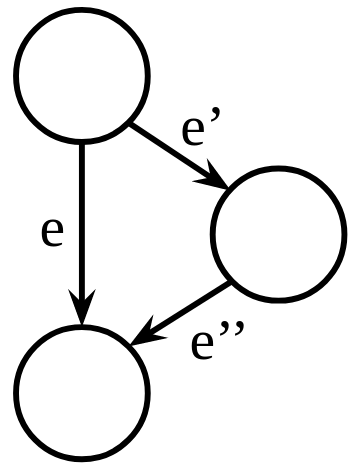
\includegraphics[height=10em]{s_on}
  \caption{$S_{on}'$, mutated $e$}
\end{subfigure}%
\begin{subfigure}{.3\textwidth}
  \centering
  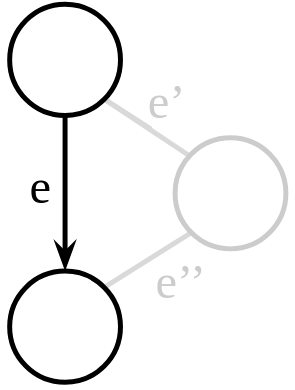
\includegraphics[height=10em]{s_off}
  \caption{$S_{off}'$, $e'$ and $e''$ disconnected}
\end{subfigure}%
\caption[The state of $S$, $S_{on}'$ and $S_{off}'$]{$S$, $S_{on}'$ and $S_{off}'$, shown in the local area around the
candidate edge $e$. Notice that while $S_{on}'$ and $S_{off}'$ are operationally identical,
(that is, contain identical copies of $e, e'$ and $e''$ and all component operations within), $S_{off}'$ is mathematically
identical to $S$.}
\label{fig:ntk_s_models}
\end{figure}

This is necessary because NTK-LRC is only useful as a comparative metric between two identically parametered-models, as
described in Section~\ref{sect:ntk_practical_concerns}. Since mutation implicitly modifies a model's operations and therefore
parameters, $S$ and $S_{on}'$ cannot be meaningfully compared. Using $S_{on}'$ and $S_{off}'$ remedies that issue, by
creating two identically-parametered models that mathematically represent a mutated and unmutated model respectively. As such,
the NTK-LRC delta induced by the mutation can then be measured, which happens in line~\ref{ntk:compute}.

If this mutation produced a favorable NTK-LRC (that is, decreased NTK and increased LRC) it is added to the set of
found good mutations $\mathcal{E}$ in line~\ref{ntk:add}. This whole process repeats until a satisfactory number of good mutations
are found or all edges have been sampled, at which point the algorithm exits the edge sampling loop (line~\ref{ntk:break}).
If any good edges are found, then the one with the most favorable joint NTK-LRC is selected in line~\ref{ntk:findbest}
as the final mutation choice. If this mutation is performable on $M$ within the available memory space
(line~\ref{ntk:iffits}), it is returned as the selected mutation. Otherwise, no edge is returned.


\section{SpiderNet Algorithm}\label{sect:spider_alg}
A variety of ways to select good mutations within models have now been covered, which means there is now a variety of ways to
grow models within the SpiderNet algorithm. As such, all necessary components for the full algorithm are present, which is
stated in Algorithm~\ref{alg:spider}.

The algorithm first starts by initializing a minimum viable model $M$ and choosing the mutation metric $\mu$. The rest
of the algorithm is very conceptually similar to BonsaiNet: the model is trained and pruned, then a number of mutations
are performed (if possible), then the whole process repeats until the model has reached sufficient size. Then the full model
trains and prunes freely until is fully trained.

\begin{algorithm}[ht]
\SetAlgoLined
Initialize `minimum viable model` $M$ as shown in Figure~\ref{fig:spider_multiin_initialization}\;
\lnl{spider_alg:mut_metric} Choose mutation metric $\mu$ and sort direction \texttt{min} or \texttt{max}\;
Let $s(x)$ refer to the VRAM size of some component $x$ as per Algorithm~\ref{alg:revised_operation_sizing}\;
Let $s_{max}$ be the maximum permitted VRAM allocation\;
Let $E_{train}$ refer to the desired number of training epochs\;
\BlankLine
\For{i in $[1, \#_{mutation\;cycles}$]}{
    \If{\upshape inter-cycle training+pruning is required/desired}{
        Reset model parameters\;
        \For {Epoch in $[1, \#_{epochs\;per\;cycle}]$}{
            \lnl{spider_alg:inter-cycle-pruning} Train + prune\;
            \lnl{spider_alg:deadhead} Deadhead\;
        }
    }
    Compute metric scores for each edge in model: $\vec{\mu} = \{ \mu(e)\;|\; e \in M \}$\;
    Choose top $n$ edges from $\vec{\mu}$ according to sort direction\;
    \For{\upshape Each chosen edge $e$}{
        \If{$s(M) + 2s(e) < s_{max}$}{
            Perform mutation on edge $e$\;
         }
    }
}
\lnl{spider_alg:intra-train-pruning} Train + prune freely for the $E_{train}$ epochs\;
\caption{The SpiderNet Algorithm}
\label{alg:spider}
\end{algorithm}


\section{CIFAR-10 Experiment Designs}\label{sect:spider_experiments}
Given the above algorithm and metrics, a variety of experiments can be designed over CIFAR-10 to evaluate their various efficacies,
the details of which are presented in this section.

\subsection{Model and Training Configuration}
Each SpiderNet model has much the same sorts of configurable hyperparameters
as BonsaiNet, and each model presented in this section adheres to the following design configuration:

\begin{itemize}   \setlength\itemsep{-.2em}
	\item \textbf{GPU Space}: 9.5 if run on an NVidia 1080Ti, 20 if using the NVidia 3090.
	\item \textbf{Scale}: 64
	\item \textbf{Sections}: [[\texttt{N}], [\texttt{R}], [\texttt{R}]]
	\item \textbf{Operations}: Same as DARTS: Identity, 3x3 Max Pool, 3x3 Average Pool, 3x3 Separable Convolution, 5x5 Separable Convolution,
	3x3 Dilated Convolution, 5x5 Dilated Convolution
\end{itemize}

The training parameters of the models like learning rate, learning rate annealing, and dropout,
are identical to those used in the BonsaiNet experiments. For exact details, see Section~\ref{sect:bonsai_training_details}.

\subsection{Evolution via Minimum Variance}
Given the promising results of the minimum variance metric as shown in Figure~\ref{fig:mutation_metrics_full_train},
this was chosen as the primary mutation metric for full training experiments. Much like the BonsaiNet algorithm
(Algorithm~\ref{alg:bonsai}), models train in cycles of four epochs. After those four epochs a deadheading pass is performed,
after which point mutation is attempted. Here, the $n$ edges with the minimum variance of their collective pruner weights
are selected as mutation candidates. Optionally, this selection can happen more granularly, instead selecting $\lfloor n/c \rfloor$ edges
from each of the $c$ cells within the model, such as to balance growth throughout each cell.
For each candidate mutation, the sum of the VRAM sizes of the new operations is
considered, and if there is sufficient VRAM space to add these new operations to the existing model, the mutation is
performed. Otherwise, the model skips this mutation and evaluates the next one. After all $n$ mutations have been evaluated
and potentially performed, all the tracked statistics are cleared. This ensures that the next batch of statistics
that is gathered will reflect the new architecture of the model.

After a number of mutation cycles the model is considered to have grown to its full size,
and trains uninterrupted to the full desired epoch count. Usually, 10 mutation cycles with three mutations per cycle (such as
to perform one mutation per cell per cycle) is
sufficient to build a model comparable in size to the 1080Ti large-cell Bonsai models,
and as such allows a fair comparison to the two. Additionally, to explore SpiderNet's capabilities in the larger
3090 domain, runs were also performed with 20 mutation cycles with three mutations per cycle. To further ensure
parity, training is performed on CIFAR-10 with identical hyperparameters to that of the Bonsai large-cell models, as discussed in
Appendix~\ref{chapter:bonsai_configs}.

\subsection{Evolution via Joint NTK-LRC Metric}\label{sect:ntklrc-evolution}
Using NTK-LRC as the mutation metric $\mu$ provides an optimal mutation to perform, if such a mutation
exists and fits in memory. Much like in Minimum Variance, this process is again split across each cell, such that
an optimal mutation is looked for and potentially performed within each cell each mutation cycle.

One interesting question that arises when using NTK-LRC as a train-free metric regards pruning;
how should it be done, considering that the differentiable pruners require training to operate? One option is to use NTK-LRC
as a slightly more expensive replacement for the normal mutation metrics and perform the training and pruning loop as
normal. Since this will be slower than using the other metrics like minimum variance that are calculated as a by-product of
the training and pruning cycle, this approach would require excellent performance in order to justify the additional time cost.

\subsection{Random Search and Ablation Studies}\label{sect:spider-random}
Following in the pattern of Bonsai and \hyperlink{cite.yu2019}{``Evaluating The Search Phase of Neural Architecture Search''}~\citep{yu2019},
a random search is devised to compare SpiderNet's ability to find good networks within the search space. In order to do this,
it is first necessary to enumerate the different `non-random' components of the algorithm. In the case of SpiderNet, there are
three: guided mutation by metric, inter-cycle pruning, and intra-training pruning, from lines~\ref{spider_alg:mut_metric},
~\ref{spider_alg:inter-cycle-pruning}, and~\ref{spider_alg:intra-train-pruning} of Algorithm~\ref{alg:spider} respectively.

Replacing guided mutation with a random measure is simple; rather than choose the edges with optimal metric values for
mutation, an edge is selected at random. Each random run then attempts to perform as many random mutations as was attempted
during a guided mutation run, typically 45 (15 cycles of three mutations each).
Not all of these mutations will actually occur due to VRAM space constraints, but both methods will have an equal number of mutation
\textit{opportunities}.

Next is inter-cycle pruning, that is, the round of differentiable pruning that occurs after each round of mutations.
To replace this with a random measure, a random selection of operations is deadheaded after each mutation cycle.
To ensure a fair comparison, the random experiment takes an existing SpiderNet run as a template for deadhead frequency, recording the
number of deadheads that occurred after each mutation cycle (line~\ref{spider_alg:deadhead} of Algorithm~\ref{alg:spider}).
The template run used in these experiments comes from a Evolution via Minimum Variance run, with the following per-cycle deadhead counts:
\begin{align*}
    \vec{dh} = [4,   2,   5,   4,   7,  13,  10,  11,  14,  13,  15,  17,  16, 24,  26,  22]
\end{align*}
\noindent Then in the random run, $\vec{dh}_i$ operations are selected at random for deadheading after the $i$th mutation
cycle. Another option is to simply not perform inter-cycle deadheading altogether as an ablation study,
to examine the necessity of its inclusion. Both options are considered in these experiments.

The final non-random component is intra-training pruning, the free pruning that occurs during training. As Section~\ref{sect:supernetevaluation}
showed, this can be immensely powerful in boosting network performance. Therefore, in order to be able to differentiate
performance stemming from mutation policy versus intra-training pruning, it is crucial to examine intra-train pruning's effects
as best as possible. To do this, the number of deadheads that occurred during the template run's
600 epochs of training are observed (line~\ref{spider_alg:intra-train-pruning} of Algorithm~\ref{alg:spider}). For the specific template
run used it was 153. Therefore, once the random runs have finished mutating, 153 operations are deadheaded at random
from the network. The network is then trained without pruning. In addition, random runs are performed that do not undergo
this final deadheading, as well as randomly grown runs that can freely prune via differentiable pruners as normal. Both of these
latter runs serve as ablation study regarding inter-cycle and intra-train pruning.

\begin{table}[ht!]
\begin{center}
\begin{tabular}{c|ccc}
    Label    & Mutation          & Inter-cycle Pruning       & Intra-train pruning \\ \hline
    Random 1 & 15 Random Cycles &  Random via $\vec{dh}$    & 153 randomly chosen \\
    Random 2 & 15 Random Cycles &  None                     & None \\
    Random 3 & 15 Random Cycles &  None                     & Differentiable \\
    Random 4 & 15 Random Cycles &  Random via $\vec{dh}$    & Differentiable \\
\end{tabular}
\end{center}
\caption[Details of the four random experiments that were run]{Details of the four random experiments that were run.}
\label{tab:spider_randoms}
\end{table}

Four different combinations of random/non-random components are chosen, and are detailed in Table~\ref{tab:spider_randoms}.
These four were chosen for their specific comparative properties. Namely, Random 1 is the pure-random run that replaces each guided component of Spider with its random equivalent, thus
serving as a purely random reference point against which to compare all experiments against. Random 2 is a pruning ablation
study, which in comparison to Random 1 will inform us of the effects of the random pruning performed. Random 3 evaluates how
well guided-pruning can mesh with random mutation. This will be useful as direct comparison against a guided-run, to determine
how much of its performance stems from the guided-mutation versus guided intra-train pruning. Finally, Random 4 evaluates how
random pruning during the mutation stage (which increases the amount of space available for mutations, therefore
leading to an increased number of mutations as more of the 45 opportunities will be successful) might benefit final
performance.


\section{CIFAR-10 Results}\label{sect:spider_results}
In Table~\ref{tab:spider_all_results} the results of the two guided mutation methods (Minimum Variance and NTK-LRC)
are compared against the four random methods. A comparison against BonsaiNet and other NAS methods is shown in Table~\ref{tab:spider_comp_performance}
later in the chapter.

\begin{table}[ht!]
\begin{center}
\begin{minipage}{\textwidth}
    \renewcommand{\thempfootnote}{\fnsymbol{mpfootnote}}
\begin{tabular}{c|c|c|c|c|c}
    Growth Strategy & Allotted VRAM & Test Accuracy    & Search Time  & Total Time & Params \\
    \hline
    Min. Variance   & 9.5      & 96.92\%          & 2.9          & 56.8       & 6.2    \\
    Min. Variance   & 20       & 97.08\%          & 6.6          & 89.8       & 7.4    \\
    NTK-LRC & \;\;6.5\footnote{This was run was performed on the 3090, the limited GPU access was due to improper VRAM deallocation of a previous experiment. However, this run demonstrates
    some interesting properties about SpiderNet's ability to perform in low allocation regimes, so is included in these results.}
                               & 96.78\%          & 5.8          & 36.2      & \textbf{4.0} \\
    NTK-LRC         & 20       & \textbf{97.13\%} & \textbf{5.4} & 74.9       & 8.8    \\
    \hline
    Random 1        & 20       & 96.96\%          & -            & 69.9       & 12.9   \\
    Random 2        & 20       & 97.03\%          & -            & 81.4       & 16.8 \\
    Random 2        & 9.5      & 96.78\%          & -            & \textbf{30.5}       & \textbf{4.0}   \\
    Random 3        & 20       & 96.97\%          & -            & 85.4       & 11.1   \\
    Random 4        & 20       & 96.81\%          & -            & 84.7       & 9.1   \\
\end{tabular}
\end{minipage}
\end{center}
\caption[Results of the nine SpiderNet runs conducted]{Results of the nine SpiderNet runs conducted. All search and run times reported in this section are given in GPU hours, max
VRAM in gigabytes, and parameter counts in millions.}
\label{tab:spider_all_results}
\end{table}

\section{Discussion}\label{sect:spider_discussion}
First, the overall ramifications of the results presented in Table~\ref{tab:spider_all_results} will be explored. Then,
 the table will be broken into specific subsets of runs whose comparisons provide interesting insights.

\subsection{Overall Results}
Of the guided mutation runs, the NTK-LRC run is superior in total runtime, search time, and accuracy. The only
place it falls short is in parameter count, which is 1.4M higher than that of the Minimum Variance run. While
 only one run of each metric was trained to the full 600 epochs due to time constraints, these performance trends
were also visible among runs that were terminated early due to runtime bugs and power failures that plagued
early Spider experiments. Interestingly, the concerns regarding the expense of NTK-LRC mutation speculated in
Section~\ref{sect:ntklrc-evolution} (that NTK-LRC would be much more expensive than Minimum Variance and thus would
need greatly improved performance to be worthwhile) ended up entirely unfounded. While mutation via NTK-LRC did provide
increased performance, mutation via NTK-LRC was actually over an hour faster than via Minimum-Variance and produced
a model that trained around 15 hours faster, and thus was pretty significantly cheaper.

Additionally, the runs of lower VRAM specification demonstrate that the SpiderNet performs well under different constraints:
apart from differing VRAM caps, these runs were configured identically. This demonstrates a versatility for performing
NAS in different hardware domains, specifically one that comes with very little need for configuration tuning. While
the configurations that performed well in the high-VRAM domain may not be optimal for low-VRAM domains (nor are
they guaranteed to be optimal even in their intended range), SpiderNet finds very good models regardless. This is exciting
from an ``applied NAS'' perspective, in that it minimizes the need to tune the algorithm to the desired domain.
This means that SpiderNet has fulfilled the goals that were outlined in the introduction of this chapter (Section~\ref{sect:spider_intro}) wherein
it was of interest to explore an algorithm free of the structural configuration tuning that weighs down fixed-structure algorithms like
DARTS or BonsaiNet.

In terms of the randomly mutated models, the non-pruned Random 2 produced the best performance,
while the purely random Random 1 produced the fastest model by runtime. This is an interesting result that ran
contrary to my expectations, which stemmed from the results of the Bonsai supernet experiments (Section~\ref{sect:supernetevaluation}).
In those, an unpruned supernet performed very well, while an identical supernet that was differentiably pruned produced
better accuracy in fewer parameters and less overall runtime. The analogue here would be Random 2 and Random 3; if the unpruned
supernet of Random 2 performed so well, it might be expected that a similarly-grown supernet that could differentiably prune would again
produce better accuracy more cheaply. However, Random 3 produced worse accuracy four hours slower than Random 2, although it
did use 5.7M fewer parameters. The same could be said about the Random 1 and Random 4 pair; all prior results about
differentiable pruning would suggest that using it as a replacament for random pruning in the training stage should increase
accuracy and decrease cost. However, Random 4 was significantly less accurate than Random 1 as well as around 15
hours slower overall.

One possible explanation to these results is that all previous pruner experiments were performed over identical
supernets, while these four random runs each have a different randomly generated structure. Given how drastically
the structure of SpiderNet models can vary (see Appendix~\ref{chapter:appendix_spider} for examples of this), the
performance differences seen may be the result of the architecture's implicit capabilities, moreso than the effects
of pruning. To fully decouple these effects, the random methods would all need to be performed over the same
randomly-mutated model, that is, pick a random sequence of mutations that are then deterministically performed
every time. However, this is a tangential line of experimentation to the main focus of the work, and thus was not
prioritized.

\subsection{Best NAS versus Best Random}\label{sect:spider_bestvbest}
The first analyzed pairing is the best guided run against the best random run, shown in Table~\ref{tab:spider_rand2}:

\begin{table}[ht!]
\begin{center}
\begin{tabular}{c|c|c|c|c|c}
    Growth Strategy & Allotted VRAM & Test Accuracy    & Search Time  & Total Time & Params \\
    \hline
    NTK-LRC         & 20       & \textbf{97.13\%} & 5.4          & \textbf{74.9}       & \textbf{8.8}    \\
    Random 2        & 20       & 97.03\%          & -            & 81.4       & 16.8 \\
\end{tabular}
\end{center}
\caption[The best random run versus the best guided run]{The best random run (Random 2) versus the best guided run (NTK-LRC).}
\label{tab:spider_rand2}
\end{table}


The most immediate conclusion that may be drawn from this is that there are only marginal accuracy differences between
the guided and random runs, with the best guided run scoring only 0.10 percentage points better than the best random run.
However, there is a large parameter difference between the two; the guided run used less than half the parameters of the
random run. Additionally, the guided run from start to finish took around six hours less than the random run. These latter
two points are particularly interesting; the whole random-search condemnation of NAS stems from random search providing
a model of equivalent accuracy and parameter count ``for free''. In any search space wherein every candidate model
has an identical count of single-path edges (DARTS, for example) this
might be a valid assumption, as the single-path restriction (see Section~\ref{sect:bonsai_search_space}) means that every
possible model contains an identical number of operations (equal to the total number of edges $e$ in the model),
meaning training times will only vary based on the computational complexity of the selected operations. Meanwhile, if
operations (and thus per-edge parameter counts) are selected from a uniform distribution (such as in~\cite{li2019}),
it is expected that the total number of parameters in any randomly generated model will also be roughly similar.\footnote{
To test this, 100,000 models were generated from a single-path, $e=57$  Bonsai search space via uniform operation selection.
    The distribution of parameter counts was highly normal (Shapiro-Wilk statistic 0.9996, p=$4.1\times 10^{-12}$),
    with a mean of 1.67M and standard deviation of 0.28M.} As a result, neither the~\cite{yu2019} or~\cite{li2019} papers
that started the random search discussion consider model training time a factor, and only the
latter mentions parameter count, albeit only to point out the equivalent parameter counts of their random and NAS models.

Meanwhile, the SpiderNet search space is entirely unbounded; models with
only three operations are valid members of the search space as are those with 300 or 3,000. Therefore, the time costs of training and parameter
counts of any such model in the space varies wildly, and is a massively important factor in determining the quality of any given model. In this
regard, the SpiderNet NTK-LRC model's speed is notable; not only does it provide an equivalently accurate (in fact,
marginally better) model than the best random-search model, this model is so parameter and time-efficient that its 5.4 hour
search time handicap is more than doubly made up over the course of training. Additionally, the NTK-LRC run only used around
15 GB of its maximum allotted 20 GB, while Random 2 used the full 20 GB, another efficiency not considered in random-search studies.


\subsection{Best NAS versus Pure Random}
Next is the comparison of the best guided run to the purely random run, shown in Table~\ref{tab:spider_rand1}:
\begin{table}[ht!]
\begin{center}
\begin{tabular}{c|c|c|c|c|c}
    Growth Strategy & Allotted VRAM & Test Accuracy    & Search Time  & Total Time & Params \\
    \hline
    NTK-LRC         & 20       & \textbf{97.13\%} & 5.4          & 74.9                 & \textbf{8.8}    \\
    Random 1        & 20       & 96.96\%          & -            & \textbf{69.9}       & 12.9   \\
\end{tabular}
\end{center}
\caption[The fastest random run versus the best guided run]{The fastest random run (Random 1) versus the best guided run (NTK-LRC).}
\label{tab:spider_rand1}
\end{table}

The purely random run compares more favorably to the best NTK-LRC run, with a faster training time and closer
parameter count, at the expense of marginally worse accuracy than Random 2. However, it still has around 4 million
more parameters than the NTK-LRC run. These results show that random search is still fairly competitive
in the SpiderNet space, albeit consistently less parameter efficient and marginally worse accuracy-wise.

\subsection{Constricted NAS versus Constricted Random}
\begin{table}[ht!]
\begin{center}
\begin{tabular}{c|c|c|c|c|c}
    Growth Strategy & Allotted VRAM & Test Accuracy    & Search Time  & Total Time & Params \\
    \hline
    Min. Variance   & 9.5      & \textbf{96.92\%} & 2.9          & 56.8             & 6.2    \\
    NTK-LRC         & \textbf{6.5}      & 96.78\%          & 5.8          & 36.2             & \textbf{4.0} \\
    Random 2        & 9.5      & 96.78\%          & -            & \textbf{30.5}    & \textbf{4.0}   \\
\end{tabular}
\end{center}
\caption[The constricted random run versus the constricted guided runs]{The constricted random run versus the constricted guided runs.}
\label{tab:spider_constrict}
\end{table}
The three runs in Table~\ref{tab:spider_constrict} comprise a set of runs where overall, top-end accuracy was less prioritized in favor of
time-efficiency (the Minimum Variance run) or parameter-efficiency (the NTK-LRC and Random 2 runs). The
latter two perform nearly identically, with the NTK-LRC taking 5.7 hours longer due to its search time
costs but requiring 3 GB less VRAM. Meanwhile, the minimum variance run has 2.2 million more parameters, but
searches very quickly and scores very highly in accuracy considering the VRAM constraints.

\subsection{Literature Comparisons}
As a final point, Table~\ref{tab:spider_comp_performance} is an extension of Table~\ref{tab:bonsai_comp_performance},
serving to compare SpiderNet against BonsaiNet and the literature. From this, it is seen that the SpiderNet search space
produces consistently excellent models that are comparable with the state-of-the-art. However,
randomly generated models in the space are also quite competitive, much more so than the random Bonsai models.

\begin{table}[ht!]
\begin{center}
\begin{tabular}{c|c|c|c}
Algorithm & Test Acc. & Params (M) & Search Hours\\
\hline
NAS-Net                     & 95.53\% 	                    & 7.1   		& 37,755 \\
ENAS Micro-search	        & 96.131\%            		    & 38.0  		& 7.7     \\
ENAS Macro-search		    & 97.11\%            		    & 4.6   		& 14.4    \\
DARTS First-order     	    & 97.00 $\pm$ 0.14\% 		    & 3.3   		& 36      \\
DARTS Second-order     	    & 97.24 $\pm$ 0.09\% 		    & 3.3   		& 96 \\
NAO (w/o weight sharing)    & \textbf{98.07\%} 	            & 144.6 		& 4,800 \\
NAO (w/ weight sharing)     & 97.07\%        	            & \textbf{2.5}  & 7 \\
ProxylessNAS                & 97.92\%                       & 5.7           & N/A           \\
ENAS/DARTS/NAO Random	  	& 96.48 $\pm$ 0.18\%			& -				& -\\
PC-DARTS                    & 97.43\%   	                & 3.6           & 2.4 \\
 \hline
Bonsai SC						& 96.83\% & 3.38 	& 11.50 \\
Bonsai Random 1 SC						& 95.32\% & 4.54 	& -- \\
Bonsai Random 2 SC						& 95.19\% & 3.68 	& -- \\
Bonsai LC1				 		& 96.69\% & 2.64 	& 2.53 \\
Bonsai LC2						& 97.04\% & 7.39	& 2.54 \\
Bonsai LC3090					& 97.07\% & 23.36 	& \textbf{1.66} \\
Bonsai LC2 (no prune, no growth)& 97.08\% & 12.04	& 0\\
Bonsai LC2 (prune, no growth)	& 97.17\% & 6.63   	& 0\\
 \hline
Spider Min-Variance             & 97.08\% & 7.4     & 6.6 \\
Spider NTK-LRC                  & 97.13\% & 8.8     & 5.4 \\
Spider Random 1                 & 97.03\% & 12.9    & -- \\
Spider Random 2                 & 96.96\% & 16.8    & -- \\
Spider Random 3                 & 96.97\% & 11.1    & -- \\
Spider Random 4                 & 96.81\% & 9.1      & --
\end{tabular}
\end{center}
\caption[CIFAR-10 statistics for all of the NAS models covered thus far, including BonsaiNet and SpiderNet]{CIFAR-10 statistics for all of the NAS models covered thus far.}
\label{tab:spider_comp_performance}
\end{table}

\section{ImageNet}
\begin{table}[h]
\begin{center}
\begin{tabular}{c|c|c|c|c|c}
 & Top-1 & Top-5 & Params (M) & Search Hours & Total Hours\\
\hline
PNAS                        & 74.2\%                        & 91.9\%            & \textbf{5.1}  & ~2,500        		& - 			\\
NAS-Net-A                   & 74.0\%                        & 91.6\%            & 5.3           & 48,000        		& -			\\
NAS-Net-B                   & 72.8\%                        & 91.3\%            & 5.3           & 48,000        		& -			\\
Regularized Evolution       & \textbf{82.8\%}               & \textbf{96.1\%}   & 86.7          & 75,600        		& -			\\
NAO (w/o weight sharing)    & 74.3\%                        & 91.8\%            & 11.35         & 4,800         		& -			\\
\multicolumn{6}{c}{\scriptsize{(all models above this line are still searching by the time SpiderNet has produced a fully-trained model)}} \\ \hline
SMASHv2                     & 61.38\%                       & 83.67\%           & 16.2          & 36			   		& -			\\
DARTS Second-order     	    & 73.3\%                        & 91.3\%            & 4.7           & 96            		& -			\\
ProxylessNAS                & 74.6\%                        & 92.2\%            & N/A           & 200           		& -			\\
PC-DARTS                    & 75.8\%   	                    & 92.7\%             & 5.3           & 91.2          		& -			\\ \hline
BonsaiNet					& 60.46\%						& 82.05\%			& 8.8			& 10.52					& 418.57   	\\
SpiderNet					& 72.27\%						& 90.60\%			& 7.9			& \textbf{3.62}			& 381.46   	\\
\end{tabular}
\end{center}
\caption[SpiderNet performance on ImageNet]{SpiderNet performance on ImageNet}
\label{tab:spider_imagenet}
\end{table}
\added{
SpiderNet was also evaluated over the ImageNet-1K dataset, following the training and data processing procedures of DARTS.
A batch size of 128 and scale of 48 was used, identical to DARTS and BonsaiNet. Again, SpiderNet searched very
    efficiently, taking just 3.6 hours to find an architecture. While still not fully competitive
    with state-of-the-art models, SpiderNet was much closer; performing some tuning and trying again could potentially
    close the gap. However, the difference between the BonsaiNet and SpiderNet performances is indicative that SpiderNet's
minimal configuration paradigm is indeed useful: the lack of available compute time by which to tune the
model configurations meant each algorithm could run just once, which in turn limited the manual intuition regarding
    dataset best practices that could be garnered. SpiderNet, by virtue of self-defining the majority of its search
configuration, managed to find a much more performant model than the heavily manually-configured BonsaiNet.
}


\section{NASComp}
\added{
SpiderNet was additionally evaluated over the NASComp-2022 datasets, again in such a way as to align with the competition
ruleset. Here, SpiderNet was allocated 12 hours per dataset of search and train time, performing 10 mutation cycles before
training for $n$ epochs, $n$ chosen to fully utilize the remaining allocated time. Each model had $c$ channels,
such that $64\times c \times h_{dataset} \times w_{dataset} = 2,097,152 = 64\times 32 \times 32 \times 32$, that is,
of equivalent dimensional product to a 32 channel CIFAR-10 model. Again, no data augmentation was used to
eliminate potential biases being introduced into policy selection due to insider knowledge of the particular
datasets. Table~\ref{tab:spider_nascomp} details SpiderNet's
performance over the datasets.
}
\begin{table}[h]
\begin{center}
\begin{tabular}{c|ccc|c}
					& \multicolumn{3}{c|}{Dataset} \\
Algorithm 			& Sadie	 			& Chester 			& Isabella 			& Total Score		\\ \hline
ResNet-18			& 80.33\% 			& 57.83\%			& 62.02\%			& 200.18			\\
NASComp-2022 Winner	& \textbf{96.08\%}	& \textbf{62.98}\%	& 61.42\%			& 220.48			\\ \hline
BonsaiNet			& 95.49\%			& 61.32\%			& \textbf{64.92}\%	& \textbf{221.73}	\\
SpiderNet			& 94.17\%			& 60.71\%			& 64.54\%			& 219.42	\\
\end{tabular}
\end{center}
\caption[SpiderNet performance on NASComp-2022 datasets]{SpiderNet performance on NASComp-2022 datasets.}
\label{tab:spider_nascomp}
\end{table}

\added{
SpiderNet's performance would have placed it in 2nd place in the actual competition, and is the third best submission
seen thus far over the datasets. Its implicit lack of design structure is likely a particular shortcoming of the SpiderNet
algorithm in this context, as the strict time-limiting of the runtime restricts the number of mutate-and-prune cycles
possible and thus the diversity of discoverable architectures. However, SpiderNet is still competitive against the state-of-the-art,
which is impressive given its minimal configuration.}

\section{Future Work}\label{sect:spider_futurework}
There is a variety of open-questions about SpiderNet's design and search space that invite exploration. Unfortunately, many of these questions would be
highly time-consuming to answer, and as such could not be explored in this work.

\subsection{Mutation Metrics}
The 11 mutation metrics explored in this work are by no means an exhaustive list of the possible ways by which
to select mutations. Metrics revolving around the dynamics of pruner weights especially constitute a limitless
area of exploration, and perhaps other summarization metrics over the last $n$ epochs similar to mean
or variance could produce interesting results. Additionally, the NTK-LRC results show that more complex measures can prove to be more
fruitful. As such, more exploration of the mutation selection metrics, as well looking at the various correlations between
different metrics and with performance could serve to further differentiate guided-mutation with random mutations.

A related question to that of mutation metric choice is the determinism of their decisions; how similar are the decisions
made by the same mutation metric over different runs? This is particularly relevant to SpiderNet, given that each
model starts at identical conditions. If there is an optimal mutation to make, an ideal metric would identify this mutation
each time, but so far none of the mutation metrics has achieved this consistency.

\subsection{Growth Strategies}
Another area with a lot of flexibility is that of the growth strategies of the models. For example, how many
cycles of pruning should be performed between each mutation stage, if any? In the case of the NTK-LRC runs, they do not require
any training to calculate their mutation metrics and so could be made significantly faster by skipping inter-cycle pruning.
However, removing inter-cycle pruning would lower the total number of mutations possible, as the model
would only ever increase in VRAM allocation. It is possible that having more mutations provides more
ability for the models to strengthen areas of concern and thus benefit performance, but alternatively
it could produce models so complex as to hinder their convergence abilities.

Another consideration in this decision is the interdependence of mutation and inter-cycle pruning.
That is to say, how are mutation choices affected by the per-edge operation choices made by the pruners, and
how well do the opposing forces of growth and pruning interact? While weight
reinitialization (Section~\ref{sect:spider_mutation_reinit}) prevents them from being entirely oppositional, judging
how well they cooperate is hard.

\subsection{Initial States and Bottlenecking}
\begin{figure}[ht!]
    \centering
  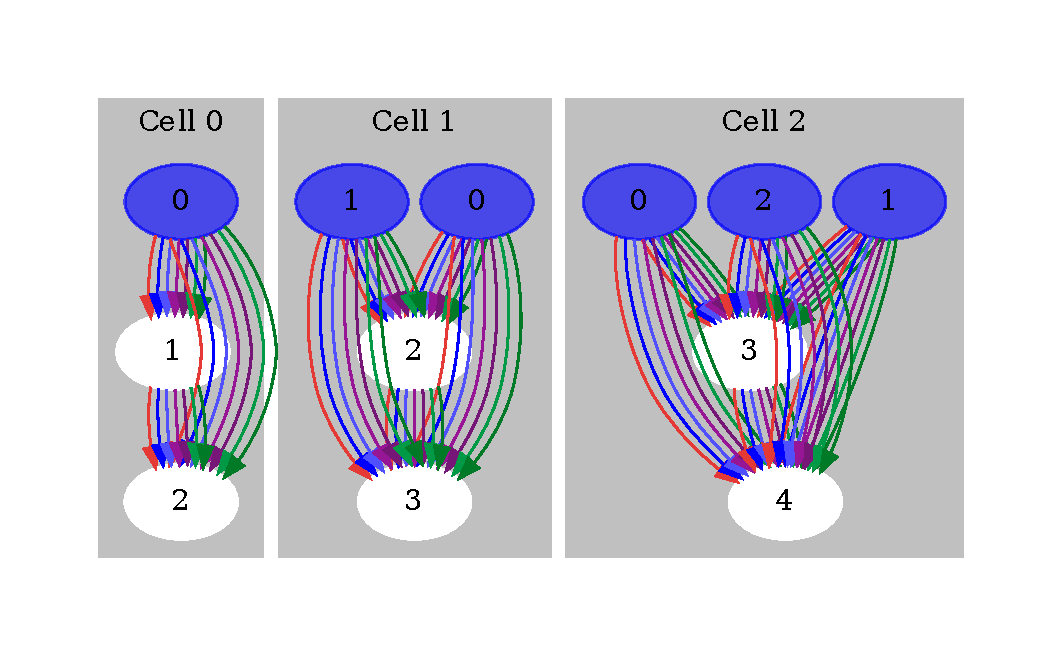
\includegraphics[width=.85\textwidth, trim={0 1.5cm 0 1.5cm}, clip]{graphs/multi_input_initial_span}
    \caption[A potential improvement to the initial state of a three cell SpiderNet model]{A potential improvement
    to the initial state of a three cell SpiderNet model, one that eliminates bottlenecking
    between input-processing and input-mixing.}
    \label{fig:spider_multiin_initialization_span}
\end{figure}

One observation that stems from comparing fully-grown models to their initial state (see Appendix~\ref{chapter:appendix_spider})
is that the division of the initial cell state into the `input-processing' section and `input-mixing' sections (for example, in
cell 1 of the initial state, edges $1\rightarrow2$ and $0\rightarrow2$ belong to the former, while $2\rightarrow3$ is in
the latter) creates a bottleneck that triangular mutations can never eliminate. That is to say that the connection
between the two cell sections is always a single node through which all information flows. For example, in Model 1 in
Appendix~\ref{chapter:appendix_spider}, Figure~\ref{fig:spider_rand0_example}, the bottleneck node
is node 18 in cell 1, and node 16 in cell 2. While it is unclear whether this is detrimental to model performance,
slightly changing the initial model state would eliminate this issue. For example, adding edges that span from each
input node to the output would provide a variety of different paths from input to output, easing the bottleneck as shown
in Figure~\ref{fig:spider_multiin_initialization_span}.

This is only one of infinite potential initial states however, and each has the ability to drastically alter the final
structure of mutated models. Studying the effects introduced by different initial states would be very interesting,
to see if the differences in eventual structure translate to performance differences.


\subsection{The False Equivalence of Random Search}
The greatest point of interest amongst of all the SpiderNet results is the triangular mutation's ability to produce
very high quality networks from minimal starting conditions. In this sense, this work is comparable to that
of~\cite{real2018}'s Regularized Evolution, which likewise grew models from minimal conditions
to state-of-the-art capabilities. Indeed, the whole concept of ``minimal initial conditions'' is directly inspired by
the ``trivial initial conditions'' described in this paper. However, what is interesting about the triangular mutation is that it can do this so quickly and consistently,
without much need to carefully consider \textit{where} it should occur. The random SpiderNet results show this
clearly, as although they are all slightly worse in various metrics than the guided SpiderNet runs, they are still comparable
in performance to the best BonsaiNet runs.

However, this is not to say that the guided-mutation work is all worthless, in fact, the opposite. Crucially,
it revealed that comparison to random search in these idiosyncratic search spaces can create a false-equivalency. If
the entire end-to-end process of finding and training a model takes as long or longer for a random algorithm than
NAS, then any accuracy similarities between the two become significantly less relevant. Section~\ref{sect:spider_bestvbest}
make this very clear; spending five hours searching is rewarded by increased accuracy, lowered VRAM, and halved
parameter counts, and then the search cost is entirely refunded and more by the increased training speed. This completely
erodes any argument that random search's comparable accuracy detracts from NAS; such an argument entirely
ignores the three other dimensions by which NAS and SpiderNet have been shown to provide benefits.

\section{Conclusion}\label{sect:spider_conclusion}
This chapter first covered SHAP and NTK-LRC, background material crucial for the design of certain components within
the chapter. Next, it described the design of SpiderNet, a Neural Architecture Search algorithm that evolves from minimal initial
conditions. A number of mutation metrics were then introduced to guide this algorithm, and were evaluated over truncated
training regimes to determine their efficacy. Additionally, a train-free mutation based around a joint Neural Tangent
Kernel and Linear Region Count metric was also explored. A number of experiments were then conducted, trialling the full
SpiderNet algorithm with different mutation metrics, along with a variety of ablation studies. These results
demonstrated that SpiderNet produces highly-competitive state-of-the-art models, but furthermore show that SpiderNet
excels against random search in a number of other dimensions beyond pure performance, namely, its superior overall runtime
and efficiency.